\documentclass{article}
\usepackage{graphicx} % Required for inserting images
\usepackage{float}
% US paper is 8.5 x 11
\usepackage[letterpaper, total={6in, 9in}]{geometry}
\usepackage{booktabs}
\usepackage{wrapfig}


\usepackage{notomath}
% switch to noto serif font
\usepackage[T1]{fontenc}
\usepackage{newunicodechar}
% declare unicode character causing problems
\newunicodechar{Ḥ}{\d{H}} % \d is dot under accent
\newunicodechar{ʾ}{’}
%#DeclareUnicodeCharacter{02BF}{‘}

\title{Princeton Geniza Project datasets}
\author{Rebecca Sutton Koeser and Marina Rustow\footnotemark}

\date{April 2025}

\usepackage[
    backend=biber,
    style=mla,
    maxbibnames=99,
]{biblatex}
\usepackage{hyperref}
\hypersetup{
    hidelinks=true  % suppress colored boxes around links
}

\bibliography{references.bib} 

% TODO: confirm that total joins are being calculated correctly

%% numbers from data
\def\totalDocuments{35,090}
\def\singleFragmentDocuments{33,544}
\def\totalJoins{1,546}
\def\totalLetter{11,202}
\def\totalLegalDocument{8,075}
\def\totalListOrTable{5,401}
\def\totalUnknown{4,181}
\def\totalLiteraryText{2,341}
\def\totalStateDocument{2,081}
\def\totalParaliteraryText{1,126}
\def\totalCreditInstrumentOrPrivateReceipt{551}
\def\totalLegalQueryOrResponsum{132}
\def\uniqueTags{2,671}
\def\taggedDimme{1640}
\def\taggedAccount{756}
\def\taggedCommunal{751}
\def\taggedIllness{691}
\def\taggedArabicScript{655}
\def\taggedIllnessLetter{646}
\def\singletonTags{1,069}
\def\totalLangauges{54}
\def\documentsNoLang{6,195}
\def\documentsAnyLang{28,895}
\def\documentsOneLang{22,333}
\def\documentsMultiLang{6,562}
\def\percentDocsMultiLang{22.7\%}
\def\percentDocsMonoLang{77.3\%}
\def\totalDatedDocs{4,375}
\def\totalDateOnDoc{4,059}
\def\totalInferredDate{316}

\begin{document}

\maketitle
\footnotetext{The authors would like to thank Mohamed Abdellatif, Amel Bensalim, Rachel Richman, Ksenia Ryzhova, Laure Thompson and Jeri Wieringa for their helpful comments and suggestions on previous drafts of this essay, and for Ksenia Ryzhova for her logistical support during the final stages of completion. }

\section{Introduction}

\begin{figure}[h!]
  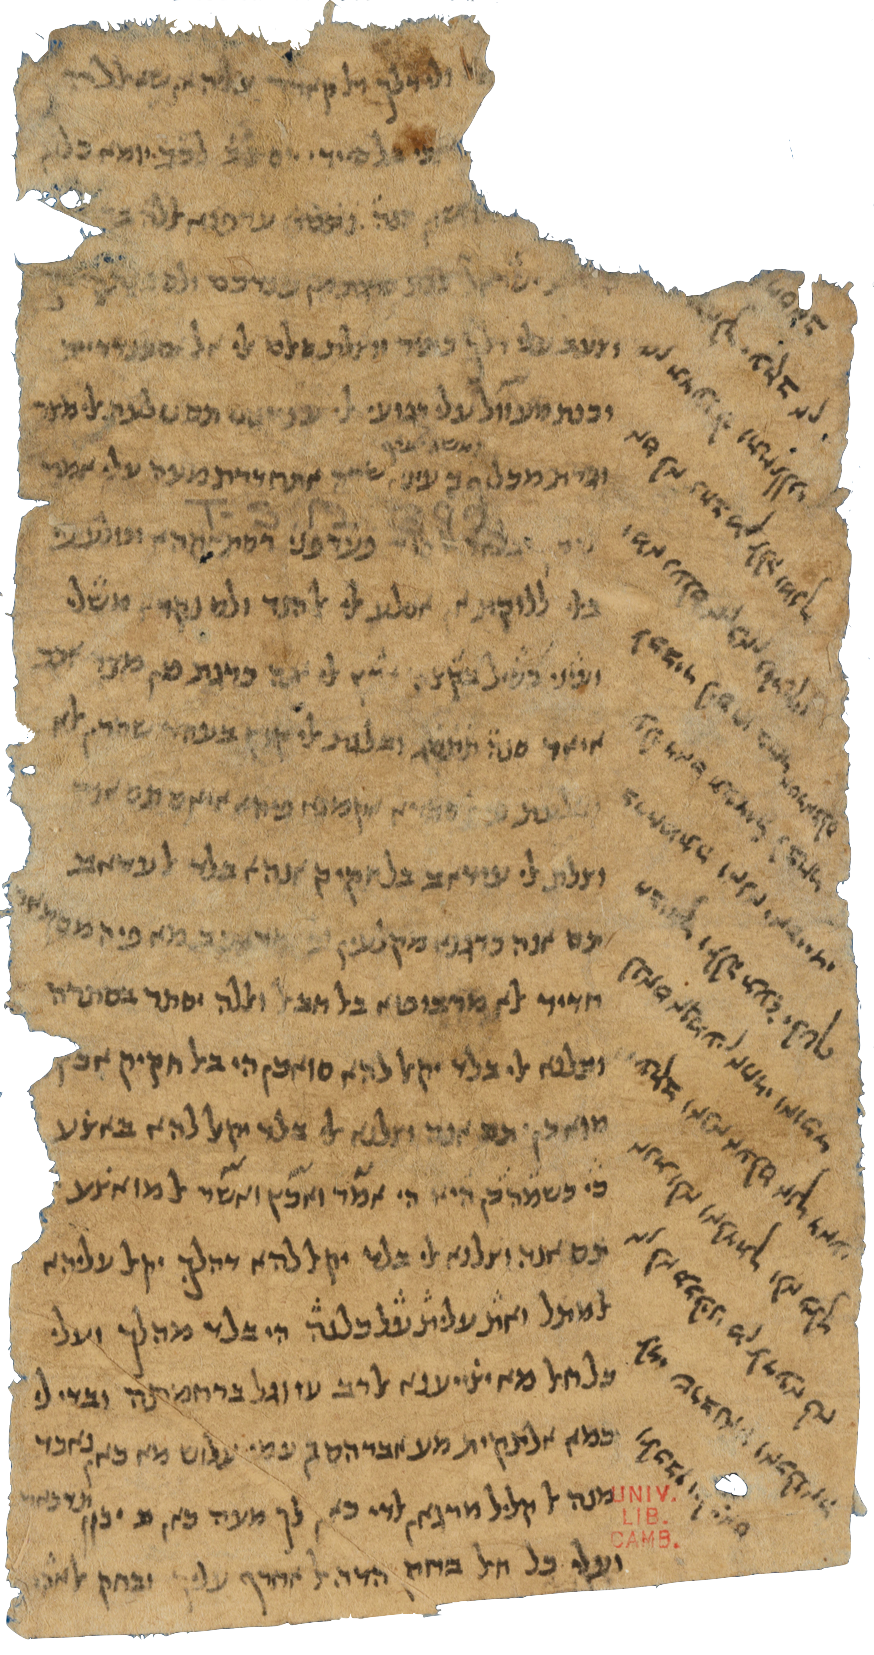
\includegraphics[height=5in]{PGPID 9690_T-S_12.392r.png}
  \centering
  \caption{Letter: T-S 12.392, Oct. 1103 CE. \textit{Princeton Geniza Project}, PGPID 9690.}
  \label{fig:pgpid9690}
\end{figure}


“Then we boarded a boat that contained not a single nail of iron, may God protect us with his shield” \autocite{noauthor_letter_1103}. Thus wrote a Libyan Jewish trader in 1103 to his brother-in-law back home. He had made it as far as Dahlak, an island in the southern Red Sea, but most of his voyage still lay before him: like many northern African traders of his generation, he hoped to make it across the Indian Ocean to the Malabar coast, where he would buy pepper and other commodities from India and farther east. Having made it up the Nile, across Egypt’s eastern desert and as far south as Dahlak, the new obstacle now before him was a type of craft he’d never seen before: one whose planks were tied together with ropes made of coconut coir. Little did he know, this was a perfectly safe way to travel; boats of this kind had been utilizing the regularity of the monsoon winds to ferry humans across the Indian Ocean since the days of the Roman emperor Nero.

\subsection{The Cairo Geniza}

The richness and detail of this trader’s story are known to us thanks to an extraordinary cache of historical sources: the Cairo Geniza, one of the densest and most coherent corpora for premodern history. A \textit{geniza} is a repository for discarded texts that according to Jewish custom cannot be casually destroyed because they are in Hebrew script or because they contain God’s name in Hebrew script. One \textit{geniza} in particular, in a medieval synagogue in Cairo, preserved hundreds of thousands of pages or fragments of pages that became available to scholars in the late nineteenth century. The texts are mostly (though not all) in Hebrew script; the ten percent of documents among them—letters, legal deeds, lists, accounts and other ephemera of everyday life—are mainly in Judaeo-Arabic, the term modern specialists use for the Arabic language written in Hebrew characters. The texts have not yet been completely cataloged, let alone published or translated; adding to the complexity of working with them is the fact that many of the texts are fragmentary, and they are now dispersed across more than sixty libraries and private collections on five continents, so that parts of the same page can be separated by an ocean.

Historical documents from the Cairo Geniza—the “documentary \textit{geniza}” for short—are especially precious because they convey unique information often not preserved in other sources, and do so candidly, without an eye to posterity: their owners never intended them to be deciphered by dogged scholars hundreds of years in the future. And a confluence of circumstances ensured that the synagogue that preserved those documents was built in the 1020s, just as Egypt was becoming the economic and cultural powerhouse of the Mediterranean and the endpoint of trade networks across the Indian Ocean. The people reflected in the documents were remarkably mobile geographically—like our Libyan with the transportation dilemma; the world the documents represent centered on Egypt, but it stretched from Spain to Sumatra. 

\subsection{The Princeton Geniza Project}

The sheer volume of new information \textit{geniza} documents offer is uncommon in premodern history. But precisely this abundance—and the fact that the texts are often incomplete and linguistically recondite—makes special demands of scholars. That’s where digitization comes in. 
Early in the personal computing era, in 1986, a Princeton-based team began digitizing transcriptions of \textit{geniza} documents to make them searchable. This was the birth of the Princeton Geniza Project (PGP), a database devoted to the documentary sources of the Cairo Geniza. In 2020, as the database approached its thirty-fifth anniversary, the authors launched a major overhaul of the database. Now, as it approaches its fortieth, we are publishing its vastly expanded data in the hope of bringing them to a wider community of digital and computational humanists and making them more tractable.

Although the PGP is a long-running project, this is the first time its data have been published comprehensively as a dataset, or separately from the interface for accessing the documents. This essay therefore describes the project’s history, explains the structure of the data and provides some context for their nuances and unevenness. We intend it as a frame of reference for anyone who wants to work with the data. 

\subsection{PGPv4}

Between 2020 and 2022, the Princeton Geniza Lab (PGL) and the Center for Digital Humanities at Princeton (CDH) partnered on a research collaboration to update the Princeton Geniza Project database. The data had become siloed and unwieldy over the years, and our goals were to streamline the database and allow researchers on the project to interact directly with it rather than through the mediation of software engineers. Especially urgent was implementing a solution for managing document transcriptions, a pain point and bottleneck for years: transcriptions are the gold standard for researchers, making it easier for historians to extract information from the documents by providing a high-quality edition of the text. We therefore modernized the database’s infrastructure by building in best practices for crediting researchers’ contributions to it, and updated the interface by including images of the documents alongside the existing transcriptions and translations. 

Over the course of a five-year period—the first two as a CDH–PGP partnership, and, after the first year, working for an additional four with Performant Software Solutions—we restructured and combined the existing project data, migrated them to a new relational database, built a transcription interface that displays transcriptions and images side-by-side, developed a way to link transcriptions to images and built modules to track the relationships among people, places and documents.\footnote{ Project charters for the first and second year of the collaboration between PGL and CDH document the significance, scope, goals, project team members, and include high-level roadmaps for the planned technical implementation for each phase. \autocite{budak_cdh_2020, rustow_cdh_2022} } 

In 2022, as we neared the launch of the first iteration of the new database, we decided to label it version 4 (PGPv4) in acknowledgment of its long history and the decades of scholarship and engineering that had gone into it, dating back to the 1980s.

The larger aim of our efforts was to accelerate research on the documentary \textit{geniza}. In this, we succeeded: in May 2021, when we launched the new admin interface, the database contained around 17,000 document entries; the ease of adding new materials and metadata allowed the team over the next two years to double the number of document entries, dramatically enriching the quality of information on these sources and accelerating the pace of research on them.

Any good engineering tool helps not only to improve data interfaces, but also to streamline team workflows. The project has allowed team members to share their research with each other and with the public in real time, and also to expand the pool of researchers to include undergraduates and even some high school students, as well as colleagues from other institutions. 

Although PGPv4 is backed by a relational database, it was always part of the plan to allow for flat data exports. Researchers on the PGP team were already accustomed to working with the project data in a shared spreadsheet, and they often made their own datasets as they gathered evidence. This publication of the data expands that capability, providing different modes and scales of access to allow for what Ryan Cordell summarizes as “zoomable, scalable, or macroscopic reading” and analysis \citeyear{cordell_what_2017}.

\section{The History of the PGP and Its Data}

The PGP datasets we are now publishing are the result of a long history of work by many researchers and software engineers.  The history of the PGP \textit{is} the research and technical work that led to these datasets, and the current data still is informed and impacted by its origins and many transformations.

\subsection{Origins of the Project}

The year 1985 was a turning point in the study of the documentary geniza. The founder of the field, S. D. Goitein (1900–85), was an extraordinarily committed, hard-working and assiduously organized researcher. When he died in January 1985, his PhD students weren’t sure the field could survive without his superhuman energy and philological expertise. Goitein had developed what he called a “lab” of research notes, transcriptions and translations, most of which remained unpublished. These included 29,000 index cards containing notes on the people, places, names, professions, objects and obscure vocabulary in the documents, as well as more than 2,000 of his transcriptions and translations. To get a sense of what this means in the life of an ordinary researcher, consider that it can take anywhere from half a day to several weeks to get a transcription or a translation right: the grammatical forms the documents use aren’t always standard, some of the vocabulary doesn’t appear in dictionaries with relevant meanings and the fragments are often faded and torn. Then there is the problem of cross-referencing words and phrases without digital aids. Goitein’s index cards, transcriptions and photocopies were his analog database. 

The staggering size of Goitein’s research archive did not make his students feel reassured about the future of their field when he died—quite the contrary. But then two of his students and a fortunate confluence of events intervened to ensure its continuation. 

Goitein had retired from the University of Pennsylvania in 1969 and moved to the Institute for Advanced Study in Princeton in 1971. Two of his students, Mark R. Cohen and A. L. Udovitch, were both then teaching in the Near Eastern Studies Department at Princeton University and were in close touch with their mentor. Then, in 1984, IBM’s Advanced Education Project donated a fleet of computing equipment to Princeton and eighteen other United States research universities in order to encourage faculty to develop classroom instruction materials that utilized personal computers. This was the dawn of the personal computing era; IBM wanted to accelerate it by embedding computers in university research. The degree to which anyone at the time imagined humanists taking advantage of it remains unclear.

In February 1985, Goitein died. In his will, he bequeathed his research archive—his “lab”—to the Jewish National and University Library (now the National Library of Israel) in Jerusalem. Before sending the material to Jerusalem, Cohen and Udovitch photocopied everything. With the indispensable help of two Princeton doctoral students in Near Eastern Studies, Paula Sanders and Amy Singer, they worked through the materials and organized and indexed them. As they did, they came up with the idea of leveraging the IBM grant to turn Goitein’s unpublished transcriptions into a full-text retrieval system. This was the birth of the Princeton Geniza Project, and of the Princeton Geniza Lab that came to house it.

Over the next ten years, Cohen, Udovitch and their doctoral students, as well as various typists and developers, created an electronic database of geniza document transcriptions using IBM software, six computer terminals and a laser printer. They managed to digitize nearly all Goitein’s published and unpublished transcriptions, as well as several hundred transcriptions by researchers whom he had trained. They also checked the transcriptions against the original manuscripts (or photostats and microfilm images of them). This resulted in extraordinarily high-quality, reliable data. This was the first version of the Princeton Geniza Project database, which our current team retroactively dubbed PGPv1, containing around 1,800 transcriptions.

To make the transcriptions searchable, the PGP team had to solve a number of unsolved engineering problems. One challenge was right-to-left, non-Latin-script search, which the technology at the time did not yet support, since Latin script was the default option for coding, indexing and display. The first solution came from a humanities computing specialist (today we would call him a research software engineer) named Michael Sperberg-McQueen who adapted existing DOS word processing software to handle both Hebrew and Arabic scripts, both of which are read right-to-left. 

A further problem—how to access the database without coming physically to Princeton—required a more complex set of solutions. Cohen remarked that at this stage of the project, as the team backed up its work on floppy disks, “we … bided our time, waiting for a way to manipulate the database and disseminate it to others \autocite[40]{cohen_princeton_2014}.

Searching the corpus was challenging as well, in part because of its size: 10 MB, laughably small by today’s standards but difficult for early PCs to index. Between 1994 and 1997, a solution arrived with an educational software engineer named Peter Batke, who took an existing program for MS-DOS called WordCruncher 4.5 and adapted it to the needs of right-to-left text. Batke possessed a combination of specializations that at the time was (in his words) “quite esoteric” \autocite{noauthor_background_nodate}. He had not only devised search solutions for other textual corpora, but also co-designed the Duke Language Toolkit, a solution for computing in non-Roman alphabets. The advantages of WordCruncher 4.5, which had been designed at Brigham Young University for indexing, searching and retrieving large textual corpora such as the collected works of Shakespeare, the Bible and the Book of Mormon, were that it could index texts relatively quickly, using small random access memory regions, and it could also produce concordances that helped researchers find terms they didn’t yet know to search for. This was a pronounced advantage for \textit{geniza} documents because of their surprisingly variable orthography. 

But then technology continued to develop apace. Batke had solved the indexing and searching problem, but he had done so in the soon-to-be-outmoded DOS environment. As of 1996, the team was still planning to distribute its data and software on CD-ROMs; the growth of the internet made this plan obsolete.

\subsection{PGPv2}

The advent of the internet led to the development of PGPv2, designed by Rafael Alvarado, Batke’s successor as humanities computing consultant at Princeton. Alvarado made the content of PGPv1 available online for the first time by migrating it to a web application he called TextGarden, which stored the documents in Extensible Markup Language (XML) and took advantage of a flexible relational model by indexing them as a network. TextGarden built on the text encoding and interface affordances of dynamic HTML, representing Hebrew and Arabic script using Unicode. Thus began the first major PGP migration from local terminals and floppy disks to a globally available website.\footnote{Our thanks to Rafael Alvarado for contributing to this write up of his work on TextGarden.} 

Migrations can be both liberating and treacherous for data. This one came with a vast improvement and some minor losses. The improvement was the Unicode text encoding system, which allowed multiple writing systems to be displayed at the same time. Before Unicode, web pages were able to display text in only one writing system at a time.\footnote{Unicode Standard Version 1.0, Volume 2 was printed in 1992; the work leading up to it included substantial efforts to support a large number of Arabic ligatures \autocite{noauthor_chronology_nodate}. Unicode and font implementations still make assumptions about languages that don't necessarily hold for the languages used in PGP materials, for instance the need to use Arabic vowels with Hebrew consonants.} This was a problem for many geniza documents, especially letters: when Jewish traders wrote to their colleagues in Judaeo-Arabic, for example, they would often write the addresses in Arabic script, since mail carriers more often than not didn't read Hebrew. Many letters are therefore in both Hebrew and Arabic script. Before Unicode, there was no way to display the transcriptions accurately. The team devised a workaround: transliterating the Arabic addresses into Hebrew script. But this misrepresented the original and also departed from best practices in the field. After Unicode, the texts could be displayed as written. (As of 2024, our team still occasionally finds addresses in Hebrew characters only to discover in comparison with the manuscript that they should be in Arabic characters—lingering artifacts of the pre-Unicode workaround.) 

There were also minor losses with the migration to PGPv2: some improper conversion of letter characters and some corruption of library shelfmarks (the equivalent of call numbers for manuscripts). These were relatively easy to fix, however. “The process of conversion was daunting,” Cohen later remarked, and “was accomplished with a certain amount of imperfection”—but he and his team eliminated most of that imperfection \autocite[43]{cohen_princeton_2014}.

PGPv2 precipitated a revolution in the field of geniza studies. Before PGPv2, the only way for researchers to access Cairo Geniza documents was via published transcriptions, leads from footnotes, Goitein’s unpublished files (in Jerusalem or Princeton) or paging through manuscripts in holding institutions. It was all needle-in-a-haystack work. PGPv2 made it possible to work from one’s home or library and to slice through a subset of the documentary geniza corpus by searching it with keywords. The Cairo Geniza was at the time believed to have preserved around 10,000 documentary texts (an estimate that later more than tripled). PGPv2 included transcriptions of 2,250 of them, and they were enough to fuel dozens of doctoral dissertations. 

\subsection{PGPv3}

The database continued to expand slowly but steadily. It did so thanks in part to a new funding stream. In the late 1990s, the Friedberg Genizah Project (FGP) in Jerusalem began working to catalogue and create digital images of all Cairo Geniza fragments, including the subset of documentary texts on which the PGP focused. The FGP’s work established for the first time what the total number of Cairo Geniza fragments was—400,000. It was still not known how many of those were documentary texts, since they hadn’t all been catalogued. So around 2004, the FGP began supporting the PGP team’s work identifying and transcribing unpublished documentary fragments. That led to the addition of another 2,000 fragments, bringing the total number of document transcriptions to 4,350.

In 2004, a new engineer joined the PGP team: Ben Johnston, an Educational Technology Consultant at Princeton’s McGraw Center for Teaching and Learning. Johnston’s contributions to the PGP began with updating the transcriptions by lightly encoding them using the Text Encoding Initiative (TEI) technical standard. He also began storing them in Bitbucket, Altassian’s Git-based source-code repository. 

But this was also the end of an era. Udovitch retired from Princeton in 2008, and Cohen retired in 2013. In 2015, Eve Krakowski and Marina Rustow replaced them as faculty in the Department of Near Eastern Studies, and Rustow became the PGP’s director. Both had been using the PGP for years, and were eager both to continue its work and to see it expand. 

Krakowski and Rustow decided, first, that it was time to find out, once and for all, how many documentary geniza texts there were. Revisiting that estimate also led to an eventual shift in the PGP’s purpose and back-end workflows. 

From the project’s origins until 2015, its goal had been to make transcribed geniza documents searchable for specialists. The project had always been geared toward specialists who knew how to read the documents, and merely needed a way to search the texts. It had never focused on creating English-language descriptions of the documents, let alone translations, since the specialists it was geared toward could do that on their own. The PGP was focused only on the most difficult of tasks: producing transcriptions. 

Because producing transcriptions was a slow and painstaking process that required many hours of paleographic and linguistic expert labor, the number of documents in the database had hovered in the low thousands for three decades. This was fine so long as the field still believed the total number of documentary \textit{geniza} texts to be around 10,000: it was a major achievement that the PGP had digitized transcriptions of nearly half of them. But no one had revisited that estimate in many years. It was due for reexamination. 

PGPv1–2 had covered only documents for which transcriptions existed. The focus of the technology behind them was therefore text search and retrieval. But PGPv3 introduced a new set of affordances, including displaying transcriptions and English-language descriptions of each document, as well as a robust set of typologies or genres. Rustow and Krakowski worked with those affordances to refocus the team’s work on generating as many English-language descriptions of documents as possible—even documents for which transcriptions didn’t yet exist. In effect, they turned the PGP from a text-retrieval system into a database of the documentary \textit{geniza}, with the goal of making it a useful tool not just for specialists but for all researchers interested in the historical material it contained. 

The result was an increase in just two or three years from the 4,350 transcriptions they had inherited from Cohen’s team to around 17,000 descriptions (see Figure \ref{fig:documents-over-time}). That rapid increase, in turn, emboldened them to revisit their estimate of the total size of the documentary corpus: they now reckoned it to be around 20,000–30,000 documents. They refocused the team’s work on identifying new documents and writing descriptions of them that even non-specialists could access.

\begin{figure}[!htb]
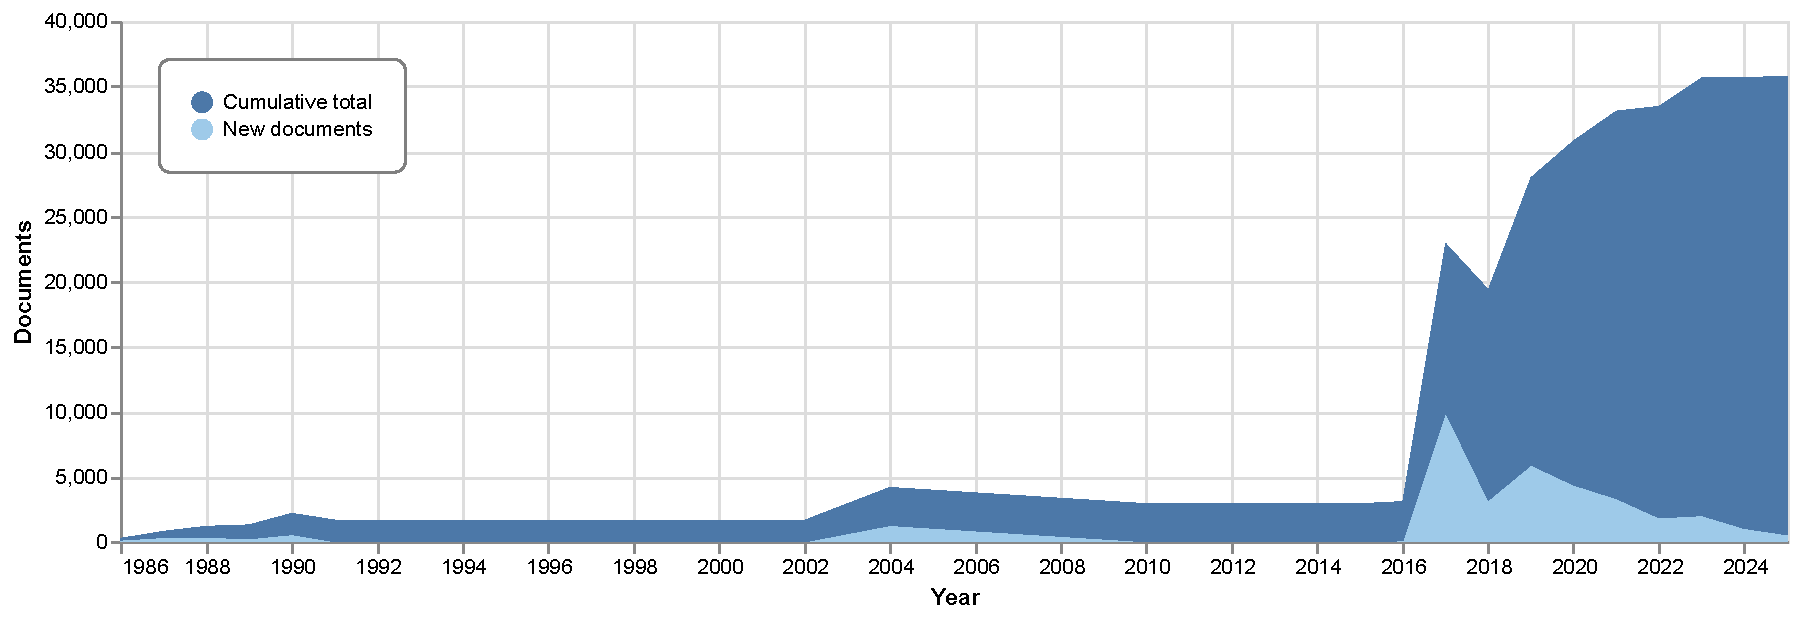
\includegraphics[width=\textwidth]{charts/docs_over_time.pdf}
\centering
\caption{Documents in PGP per year with cumulative total. The spike between 2016 and 2018 is due to the shift from transcription to description.}
\label{fig:documents-over-time}
\end{figure}

Beyond the new estimate, there were other implications of the shift from transcriptions to descriptions. Writing descriptions allowed researchers the latitude to add documents to the database even if they couldn’t decipher every word of them. And adding difficult documents to the database would also, the team hoped, enable researchers to find them more easily and come up with their own transcriptions. 

Moreover, documents can become easier to decipher in batches (we’ll return to this point below). By reading dozens of sales contracts, for instance, you can clarify the textual structure and patterns they use, and once you’ve read fifty sales contracts, you can anticipate what even a fragmentary or faded contract should be saying in the bits you can’t decipher. Even when the handwriting is difficult or the document is riddled with holes and abrasions, find similar documents and you can fill in the blanks. By capturing as many documents as possible and grouping them into types, Krakowski and Rustow hoped not just to accelerate the addition of new documents to the database, but to arrive at a more realistic picture of the documentary geniza and its scope.

To support the rapid expansion of the database, Johnston rebuilt the system to ingest descriptive metadata from a Google spreadsheet. Now instead of changes to the database going through the project directors and two or three trusted researchers, the directors gave roughly a dozen researchers access to the spreadsheet so they could add or edit descriptions—a great improvement in the flexibility and collaborative power of the PGP. 

That collaborative power extended not only to individual researchers, but also to other institutions. The scope of the PGP expanded with the addition of a large batch of records that the Cambridge University Library had created in its dedicated Genizah Research Unit, which since the early 1970s had employed PhD- and postdoctoral-level scholars to write tens of thousands of descriptions of \textit{geniza} fragments, around 7,000 of which were documentary texts. In 2017, the Cambridge team graciously gave Rustow their document descriptions and the PGP team ingested them wholesale (giving credit to CUDL), checking and expanding them over the subsequent years. The team also received metadata from the FGP database, which resulted in more than 2,000 new descriptions.\footnote{These FGP descriptions were crowd-sourced, so rather than ingesting them wholesale, the team hired Amir Ashur to review and revise them, a task he accomplished in 2022–23.
} PGPv3 resulted in a massive and relatively painless expansion of the database, bringing the total number of documents well beyond the historical estimate of 10,000. 

But then the expansion of the PGP’s focus and data pushed its infrastructure to the breaking point. The Google Sheets metadata spreadsheet had made adding document descriptions astonishingly easy. But the number of entries grew large enough that the spreadsheet became too unwieldy to load on every machine. The team now had an urgent need to build another system. Rustow, Krakowski and Johnston recognized that they would eventually need to rebuild the system. 

Once they knew they would have to rebuild the system, they began to take stock of the problems in PGPv3. 

In addition to the cumbersomeness of the metadata spreadsheet, there was another workflow challenge: it was still cumbersome to make even minor edits to the transcriptions. If researchers found a typo or came up with a better reading of a text, the protocol had long been that they sent emails to the director, who in turn passed the edits on to Johnston, who meanwhile had taught himself to read the Hebrew and Arabic alphabets and inserted the changes himself. Johnston had simplified this cumbersome process by giving Rustow, Krakowski and two of their research assistants access to the Bitbucket repository so they could edit the texts directly. But Bitbucket didn’t handle right-to-left text well, and the process was still cumbersome enough to discourage editorial changes. 

Rustow and Krakowski began consulting with the Center for Digital Humanities in 2017. It was only then that they became aware of the long-term need for better project documentation, stability and sustainability as they contemplated what PGP would look like over the next decade (or four). These were the immediate motivations for the PGL-CDH research partnership that began in July, 2020.

\subsection{PGPv4}

The lead researchers on PGPv4 were Rebecca Sutton Koeser, who led the software design and implementation team, and Marina Rustow, who led the research team. They worked together with another software engineer (Nick Budak, replaced in 2021 by Ben Silverman of Performant Software Solutions), a UX designer (Gissoo Douroudian, replaced in 2022 by Chelsea Giordan of Performant Software Solutions) and PhD students in geniza studies and related fields who served as project managers (Stephanie Luescher [2020-1], Rachel Richman [2020-present], Zohar Berman [2021-2], Ksenia Ryzhova [2022-present] and Amel Bensalim [2023-present]). The expansion of the team created two needs that the PGP had never had to face before: regular meetings and intensive documentation. Thanks to the CDH’s experience with similar partnerships, they were able to put the new team workflows in place relatively quickly over the second half of 2020. (In what follows, “we” refers to this expanded team.) The collaborative effort required the engineers on the research team to learn the basics of geniza studies, and the geniza researchers to learn about data modeling and software engineering workflows.

As we designed PGPv4, the first and most important decision we made was to migrate the data from a flat model to a relational database. After three months of weekly conversations on data modeling, we knew how we wanted to structure it: at its core, there needed to be a many-to-many relationship between fragments and documents. 

A fragment is the physical piece of paper or parchment, usually with its own shelfmark, the identifier used by the owning institution to reference the material object); a document is a discrete textual unit, such as a letter, contract or list.\footnote{In some cases, libraries gave a single shelfmark to unrelated fragments, typically when they were small and needed to be encapsulated within the same “multifragment” page of large binders. Multifragment shelfmarks can be found at Cambridge for very tiny fragments that so far haven’t been catalogued in the PGP, and at JTS for larger fragments, many of which are documents in the PGP.} Often a fragment was covered with writing: medieval scribes were nothing if not frugal. Paper and parchment were not exactly scarce, but they weren’t cheap, either, and writers often reused materials, flipping over a letter they had received to scribble down a financial account, or drafting a legal document on the back of another legal document, or writing a letter around the text of an official communiqué that a state bureaucrat had scrapped and shredded. We wanted to be able to display each of the documents on a single fragment discretely, but without losing its relationship to the other document(s) on the same piece of paper or parchment. 

The converse situation was nearly as common: just as each fragment could contain more than one document, some documents were comprised of more than one fragment. This was because many documents were torn in the jumble of the synagogue geniza chamber, and fragments containing parts of the same document ended up in different libraries, or even in the same library under different shelfmarks. There are thousands of cases of the top half of a page in, say, New York and the bottom in Oxford, or the right and left side of the same page both in Cambridge, but under different shelfmarks and unbeknownst to the librarians. When specialists reunite these pieces of what used to be a single page, they call it a “join,” and finding one is a cause for celebration—perhaps not as momentous as discovering a new subatomic particle, but worthy of a champagne toast, satisfying in the same way as completing a puzzle or staving off just a little bit of entropy in the world. 

A document can occupy more than one fragment, then, and a fragment can contain more than one document. That many-to-many relationship was the basis of our decision to build a relational database. 

Doing so required us to walk away from a longstanding informational hierarchy that the field had taken for granted: that there is a base unit of analysis, whether the fragment or the document; one always seemed to be the star of the show. This implicit hierarchy had been baked into previous printed scholarship and digital tools, structuring the display of information in different ways. Libraries, since they are custodians of physical objects, tended to privilege the fragment. The Friedberg Genizah Project database followed suit and displayed images of fragments, since it was born as an imaging project. But scholarly editions focused on textual units such as documents, since their task was to present and analyze coherent textual units. The PGP, since it had been developed by historians, also tended to favor the document, but we were also aware that doing so entailed some loss of information: for example, if you had a legal document on one side of a fragment and a business letter on the other, they were two different entries in PGPv1–3, and the connection between the two wasn’t obvious. We wanted to make it clearer: the author of the second document had somehow gotten their hands on the first, and a document changing hands is relevant information to a historian. 

Using a relational data model allowed us to sidestep this longstanding hierarchy and acknowledge the importance of both depending on the context. The fragment is what you request when you go to a library or search for a digital image; the document is what you transcribe when you create a text edition. PGP needed to account for both, and for the relationship between them. 

%% TODO: do we want a diagram ? the one we have doesn't accurately represent things

The many-to-many relationship between documents and fragments is but one example of our underlying data structure. It is a representative example in that it demonstrates the necessity of understanding something about geniza documents and the history of research on them in order to work with the data. In the next part of this essay, we will shift from the history of the project and the challenges that drove its software development over the years to the nature and structure of the current PGP datasets.

\section{The nature and structure of the datasets}

The process of rebuilding the PGP began in July 2020 and is now nearly complete—a five-year process from start to finish. But the rewards came long before the work wrapped up. In May 2021, we launched the new admin interface, and the pace at which the team added documents to the database rapidly accelerated. A good research infrastructure should encourage and inspire research, and ours quickly did just that, facilitating the production of robust datasets. 

The PGP datasets that this essay describes are exported from the PGPv4 web application as multiple flat, tabular data files. They are exported from the PGPv4 web application, which is implemented in the Django framework and is backed by a relational database (PostgreSQL). Familiarity with the structure of the underlying database and choices made in modeling the data should make it easier to understand and work with the exported data, and to recombine the data. 

\begin{figure}[!ht]
  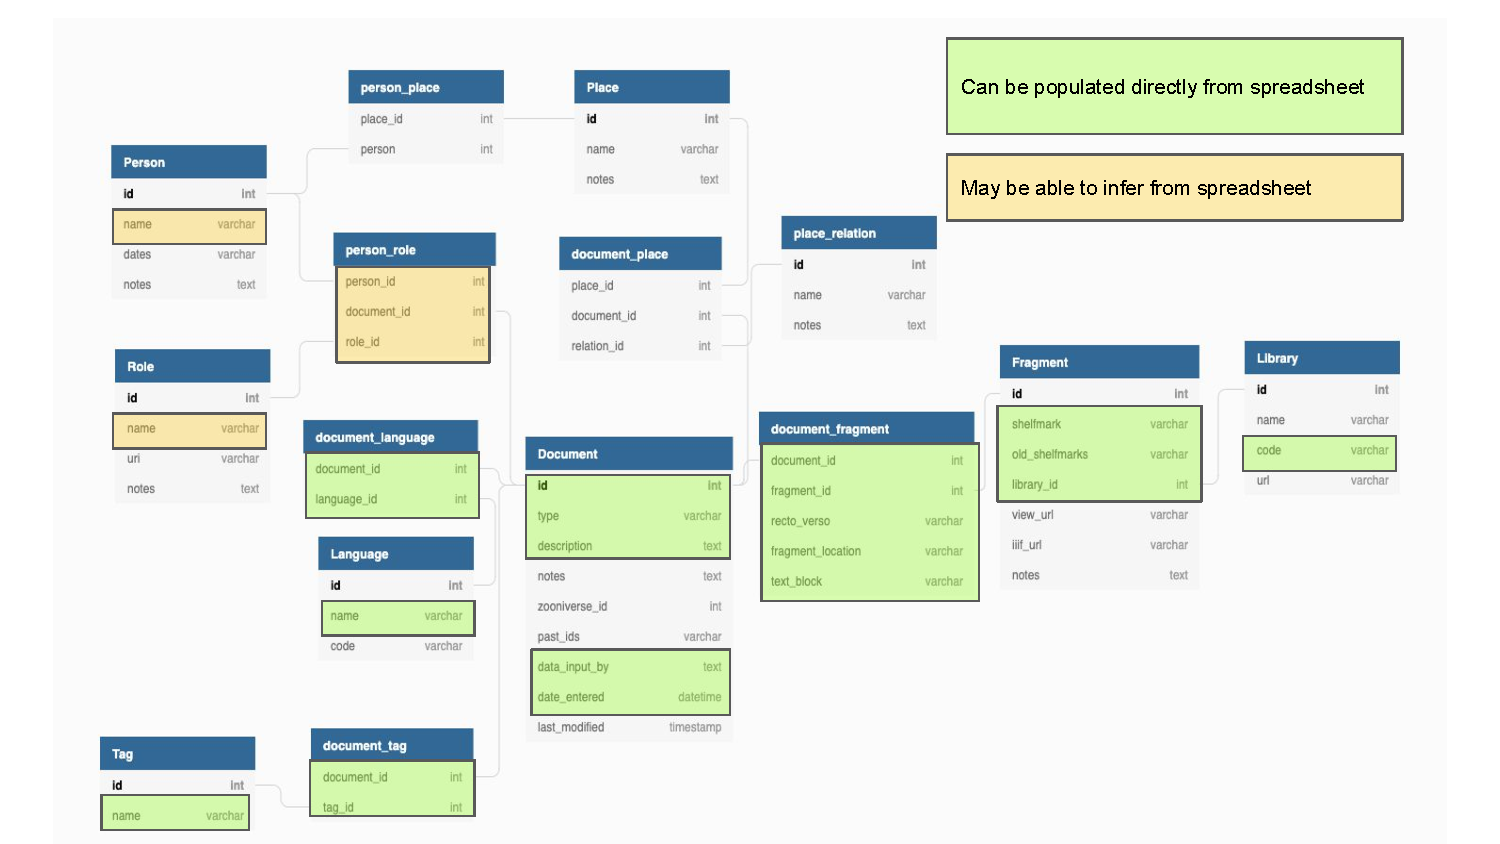
\includegraphics[width=\textwidth]{db-diagrams/pgpv4_dbdiagram_import.pdf}
  \centering
  \caption{Preliminary database diagram from project planning documents, October 2020. Annotations indicate proposed data migration from PGPv3 metadata spreadsheet.}
  \label{fig:pgpv4_dbdiagram}
\end{figure}


\subsection{Fragments and Documents}

In PGPv4, each fragment is correlated with a shelfmark, a holding institution, and a collection within that institution. Documents are correlated with other kinds of structured information, such as descriptions, tags, and the languages in which the documents are written. This relational data structure makes it easier to find and access documents that are written on the same fragment. In the PGPv4 web interface, documents written on the same fragment are linked under “related documents.”

Fragments are identified by the shelfmarks assigned to them by their holding institutions. Documents have unique numeric identifiers we call PGPIDs. Shelfmarks rarely change; when they do, PGP includes both the new and the old shelfmark. PGPIDs change less rarely: sometimes duplicate documents are found and merged into a single PGPID. The PGPv4 web application tracks both historic shelfmarks and old PGPIDs to find records when identifiers have changed, but that information is not currently included in the data exports.

\begin{figure}[!hbt]
  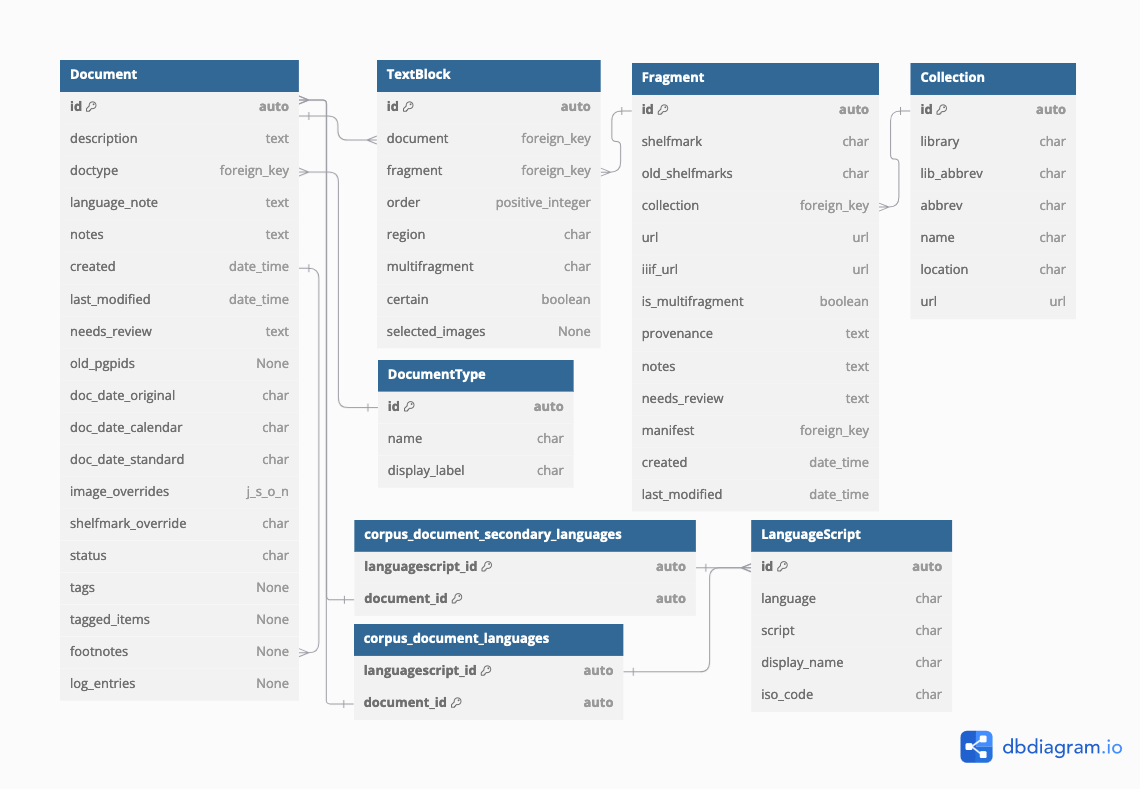
\includegraphics[width=1\linewidth]{db-diagrams/pgp v4.19 documents.png}
  \centering
  \caption{Database diagram showing relationships between documents and fragments.}
  \medskip
    \small
  Generated from models in  PGP Django codebase v4.19. Translation text fields are omitted for simplicity.
  \label{fig:pgpv4_db_documents}
\end{figure}

In SQL, a many-to-many relationship requires an additional database table to track pairs of related objects. A minimal implementation of this relationship would be a list of document and fragment id pairs, where each identifier occurs once for each related object; a document written on a single fragment would have one entry, where a document written across two fragments would have two entries with the same document id and two different fragment ids.  PGPv4 stores additional information about the relationship between a document and a fragment in this connecting table (refer to "TextBlock" table in Figure \ref{fig:pgpv4_db_documents}). These extra fields enable researchers describing documents to explicitly specify the order of fragments, add notes to identify the specific portion of a multifragment, or even to indicate an uncertain relationship. 

%\begin{wraptable}{l}{2.75in}
\begin{table}
\begin{center}
\caption{Documents by number of fragments}
\label{table:docs_per_numfrags}
\begin{tabular}{rrr}
\toprule
{Fragments} & {Documents} & {\%}\\
\midrule
1 & 33,644 & 95.60\% \\
2 & 1,178 & 3.35\% \\
3 & 183 & 0.52\% \\
4 & 87 & 0.25\% \\
5 & 45 & 0.13\% \\
6 & 24 & 0.07\% \\
8-64 & 25 & 0.07\% \\
\bottomrule
\end{tabular}
\end{center}
\end{table}
%\end{wraptable}

The majority of PGP documents—\singleFragmentDocuments, or more than 95\%—are written on a single fragment. They are not joins, and so are simple from a data modeling perspective. There are \totalJoins\space documents that are joins, most of them between two fragments, and some among more than two fragments (see Table \ref{table:docs_per_numfrags}). A small set of outlier documents are correlated with an unusually large number of fragments — 32, 34 and 64 respectively; these are multipage documents, and they are all notebooks containing the legal archives of a courtroom.


\begin{figure}[!hbt]
  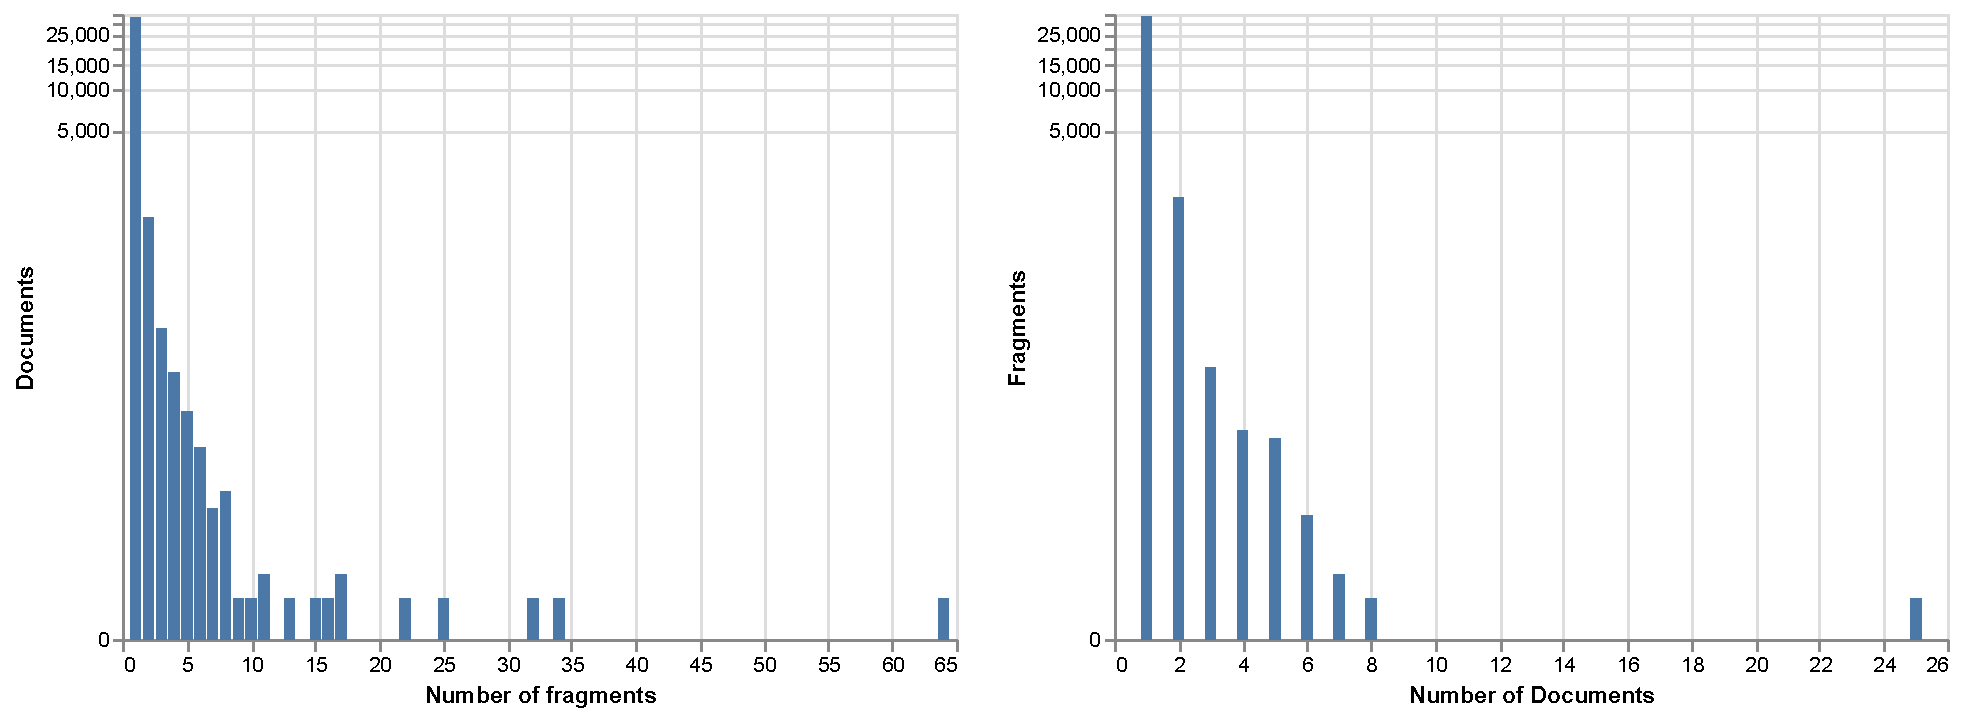
\includegraphics[width=1.0\linewidth]{charts/docs_frags_2up.pdf}
  \centering
  \caption{Left: Documents by number of fragments. Right: Fragments by number of documents.}
  \label{fig:docs_per_num_frags}
\end{figure}

% \begin{figure}[hbt]
%   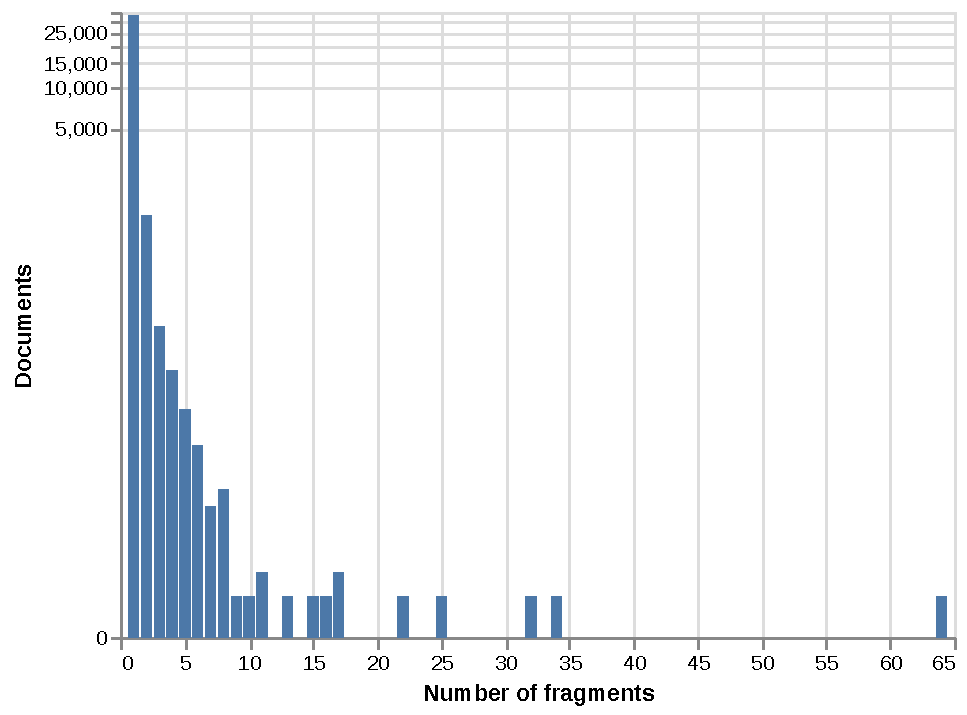
\includegraphics[width=0.5\linewidth]{charts/documents_per_num_frags.pdf}
%   \centering
%   \caption{Documents by number of fragments}
%   \label{fig:docs_per_num_frags}
% \end{figure}

% \begin{figure}[hbt]
%   \centering
%   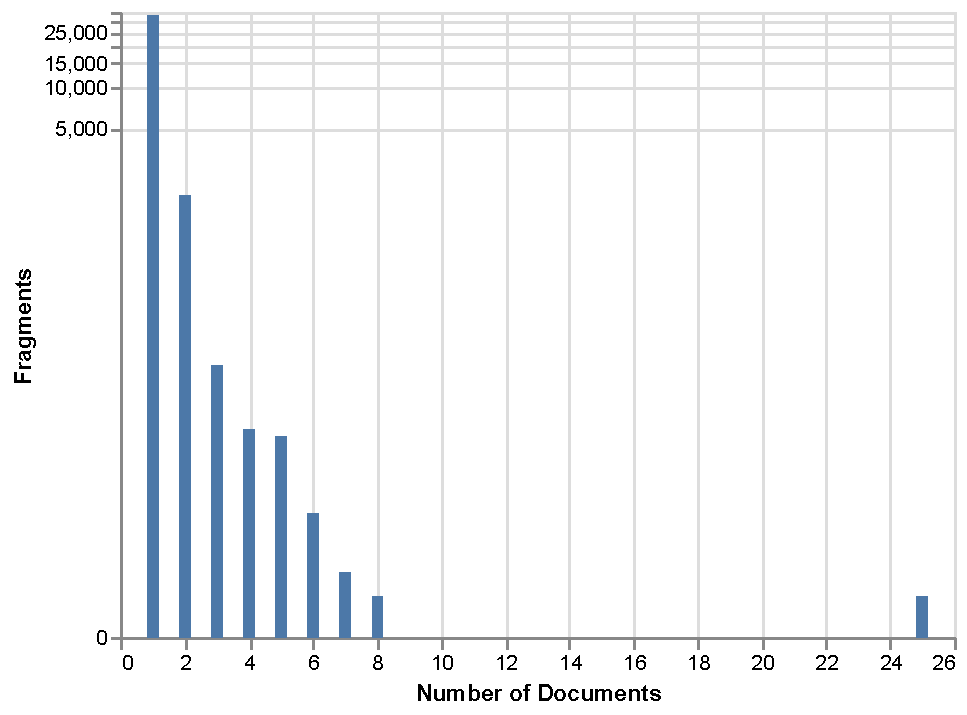
\includegraphics[width=0.5\linewidth]{charts/fragments_with_num_docs.pdf}
%   \centering
%   \caption{Fragments by number of documents}
%   \label{fig:frags_by_num_docs}
% \end{figure}

If we flip the question and ask how many fragments contain more than one document, again we find that the majority (nearly 90\%) contain a single document.

The more complicated cases provide an opportunity to draw insights beyond the textual and visual contents of individual documents. The co-occurrence of different texts on the same fragment enables scholars to trace new histories of paper and parchment circulation and reuse. For instance, two petitions to the Fatimid ruler Sitt al-Mulk \autocite{noauthor_state_1024, noauthor_state_1021} were glued together by a Jewish scribe in need of a long vertical scroll on which to copy a liturgical text. By making the relationship between documents and fragments more explicit and easier to navigate, PGPv4 makes it easier to work across related documents and reused fragments.

\subsection{Types, Descriptions, and Tags}

Each document entry in the database includes three main metadata components: types, descriptions, and tags. Every document has a description, even if it is short; nearly all documents have a type.

\begin{figure}[!hbt]
    \centering
    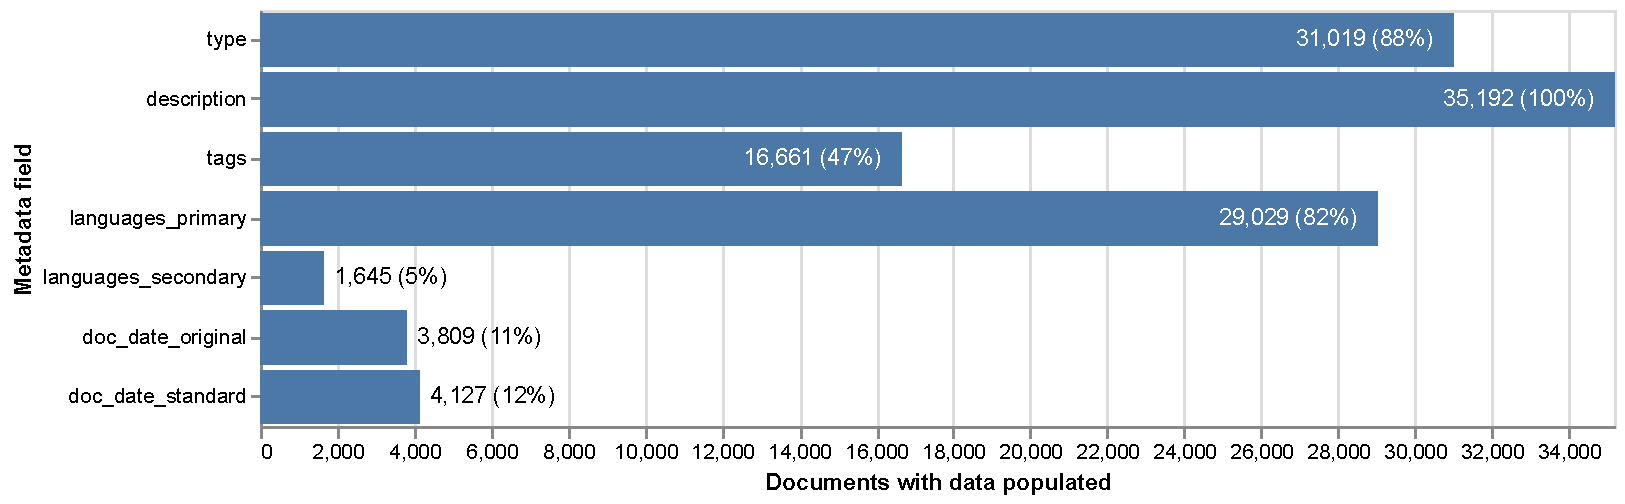
\includegraphics[width=1.0\linewidth]{charts/metadata_available.pdf}
    \caption{Availability of metadata fields across documents}
    \label{fig:metadata-status}
\end{figure}

\textbf{Types} are ways of categorizing documents according to their textual structure. Each document is categorized under a single type. PGP uses an intentionally simplified set of categories that Krakowski and Rustow developed over the course of several years of discussion and workshopping with other colleagues. The simplicity of this typology makes it easier to enter new documents into the database and to group like with like. 

\begin{enumerate}
    \item     \textbf{Credit instrument or private receipt}: letters of credit, commercial receipts, records of debt, records of payment. Excluded: financial transactions mentioned in legal documents.
    \item \textbf{Legal document}: bills of sale, testimonies, quittances drawn up by courts (as distinct from private receipts), marriage contracts, divorce deeds, summaries of court cases.
    \item \textbf{Legal query or responsum}: special types of legal texts either describing a case in order to solicit a legal opinion, or rendering a non-binding legal opinion on it.
    \item \textbf{Letter}: correspondence between business associates and/or family members; official administrative letters from leaders of Jewish communities.
    \item \textbf{List or table}: commercial accounts, grocery lists, genealogical lists, charity distribution tables, inventory lists, jottings in list or tabular form.
    \item \textbf{Literary text}: not documents, but we include them in the PGP on a case-by-case basis if they capture significant historical information relevant to our documentary texts, for instance poems dedicated to known individuals; historical chronicles.
    \item \textbf{Paraliterary text}: a confusing name inherited from the field of papyrology. These are documentary texts such as amulets, calendars, magic spells, prescriptions and recipes.
    \item \textbf{State document}: official communiqué to or from government officials, including decrees, petitions, internal memoranda and tax receipts.
    \item \textbf{Unknown type}: illegible, unidentified, or uncategorized text that requires further study.
\end{enumerate}


\begin{figure}[!hbt]
  \centering
  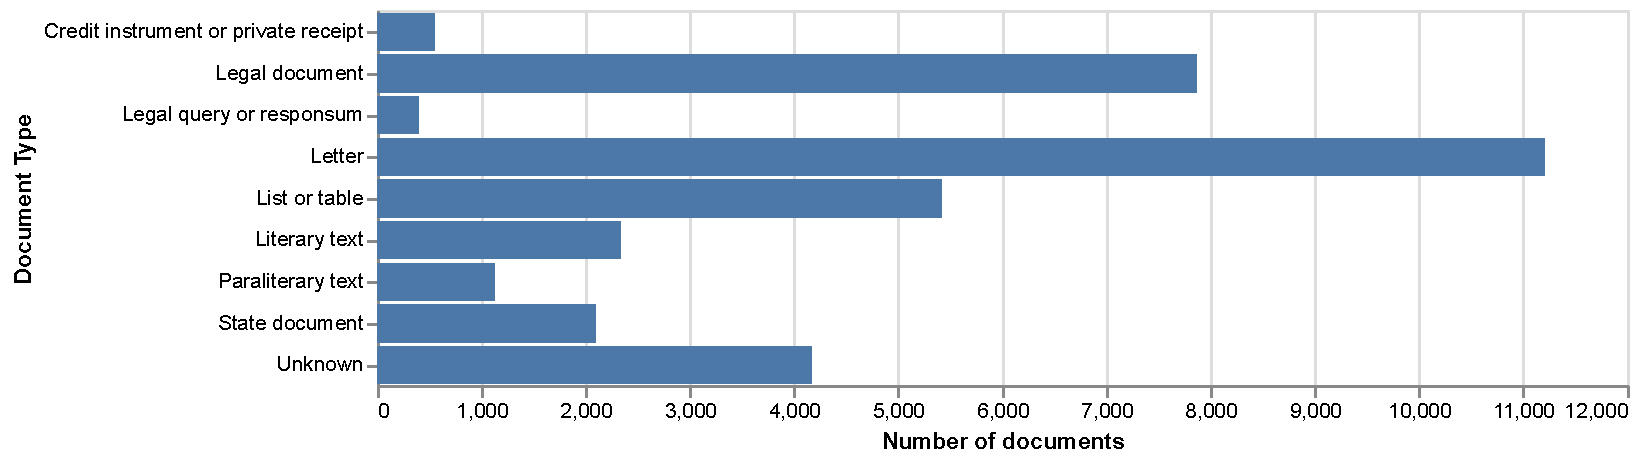
\includegraphics[width=1\linewidth]{charts/document_types.pdf}
  \caption{Documents by Type}
  \label{fig:document_types}
\end{figure}

This nine-part typology addresses the need to reduce friction at two key stages of working with the data: entering a document for the first time and transcribing it. It reduces friction at the data-entry stage by avoiding complex decision trees. Although there are many more than eight templates that the scribes of the documents were following (or devising on the fly), when entering a document for the first time, picking through a massive list of document types places an undue burden on the researcher. These nine types cover nearly all the existing cases. 

It reduces friction at the transcription stage by making it easier to find similar documents for reference, allowing researchers to compare documents easily in order to facilitate transcription. If you’re faced with the task of transcribing a document that is faded, torn or full of holes, looking at similar documents will help you fill in the blanks. True, scribes tended to use formulaic phrases the way experienced chefs use ingredients rather than slavishly following recipes; but the eight-part typology is a way of bringing similar documents together without overdetermining their shared features or misrepresenting the way scribes worked.

There are currently \textbf{\totalDocuments} documents in PGP. The most common types are letters (\textbf\totalLetter) and legal documents (\textbf{\totalLegalDocument}; see Figure \ref{fig:document_types}). The current dataset includes \textbf{\totalUnknown} documents of unknown type, which usually means they have not yet been cataloged and described, or else that don’t fall into existing categories. 

All documents have \textbf{descriptions}, although some of them may be short. These are English-language summaries of the main contents of a document. (Some documents also have Hebrew-language descriptions culled from existing Hebrew-language scholarship.) Descriptions don’t follow a strict template, and they can range in size from terse to expansive. Most are brief, with an average of 271 characters and 45 tokens. They are generally structured as an inverted pyramid putting the main information—author, recipient, locations, dates—followed by the details, for instance: 

\begin{quote}
Letter from Nahray b. Nissim in Alexandria to his uncle Abū l-Khayr Mūsā b. Barhūn al-Tāhartī in Fustat. Dating (Gil): 11 or 12 April 1051. Nahray reports among other things that he had forgotten to bring his capitation tax receipt ‘for the year 441’ on a business trip. \autocite{noauthor_letter_1050}
\end{quote}
Descriptions are, by their nature, one place where the data’s unevenness emerges. Sometimes descriptions are short due to a lack of existing research on a document; in other cases, they are short because the documents entered into the database in the 1990s, before the team started including descriptions for non-specialists. Some of the longest descriptions are of documents that the PGP team identified recently, and they wanted to put as much information about them as possible into the database for future researchers. Others are for the opposite reason: because they’ve been in the database for a long time or have received copious attention in scholarship and accumulated a long trail of research and publications. 

\textbf{Tags} are equally uneven. They are essentially free-text, and there is no restriction on the number of tags that can be applied to a document (although the interface has an auto-complete function to help researchers select preexisting tags rather than multiplying them needlessly). Existing tags do not reflect a concerted effort by the team to tag all our documents; rather, they represent our current and past research interests. 

For example, one of our research team members, Alan Elbaum, wrote his master’s thesis on people’s descriptions of their physical ailments, so there are a great number of tags in the database related to illness. Since it is impossible to anticipate all the possible questions that future historians will bring to geniza documents, our goal is not to produce tags for some theoretical future researcher, but to flag themes or individuals of interest. Tags don’t, then, represent the current state of documentary geniza research; they are less like library subject headings and more PGP researchers’ post-it notes.

The datasets contain \uniqueTags\space unique tags, of which \singletonTags\space are used only once. Some of the most commonly used ones are \texttt{\#account} (used for \taggedAccount\space and flagging a future attempt to decipher traders’ accounts); \texttt{\#communal} (used for \taggedCommunal\space documents reflecting the organizational levels of the Jewish community); \texttt{\#illness} and \texttt{\#illness letter 969-1517}  (used for \taggedIllness\space and \taggedIllnessLetter\space documents, respectively). 

\subsection{Languages and Scripts}

\begin{wraptable}{r}{3in}
\caption{Common and Unidentified Languages}
\label{table:langs_docs}
\begin{tabular}{lr}
\toprule
Language/Script & Documents \\
\midrule
Judaeo-Arabic & 15,885 \\
Arabic & 9,539 \\
Hebrew & 7,644 \\
Aramaic & 1,756 \\
Greek/Coptic Numerals & 879 \\
Ladino & 368 \\
\midrule
Unidentified language and script & 40 \\
Unidentified (Hebrew script) & 22 \\
Unidentified (Latin script) & 8 \\
\bottomrule
\end{tabular}
\end{wraptable}

Geniza materials are written in a variety of languages and scripts, including Judaeo-Arabic (a range of Arabic dialects and registers written in Hebrew characters), Hebrew, Aramaic and Ladino (a range of medieval Romance dialects and registers written in Hebrew characters).

To simplify the data structure, we modeled languages and scripts as a single entity. For instance, Judaeo-Arabic is a single entity, not Arabic language and Hebrew script. Table \ref{table:langs_docs} shows the languages that appear on the largest number of documents. (Documents often use more than one language, so these totals may include the same documents more than once.) 

One special case on the table is Greek/Coptic Numerals—not a language but a writing system specifically for numbers. Many scribes who knew neither Greek nor Coptic wrote alphanumerals derived from Coptic (and, in turn, from Greek). Since they were part of what was effectively a mercantile notation system, we thought they were worth tracking separately. Greek/Coptic Numerals is therefore a language/script category distinct from either Greek or Coptic.

We also include a few unknown languages and scripts, and these may be of interest to scholars who want to tackle a challenge. Table \ref{table:langs_docs} includes unidentified or partially unidentified languages and scripts, with the associated number of documents. These designations indicate that a researcher has examined the document and either was unable to read or identify the script or could identify the script but not the language it was used to write.

Because the authors of Geniza documents often employed a mix of languages, our data model allows documents to have multiple languages. Of the \documentsAnyLang documents with language information, \documentsMultiLang (\percentDocsMultiLang) have multiple languages. The most common combinations are Judaeo-Arabic with Hebrew and Judaeo-Arabic with Arabic. 

\begin{figure}[!hbt]
  \centering
  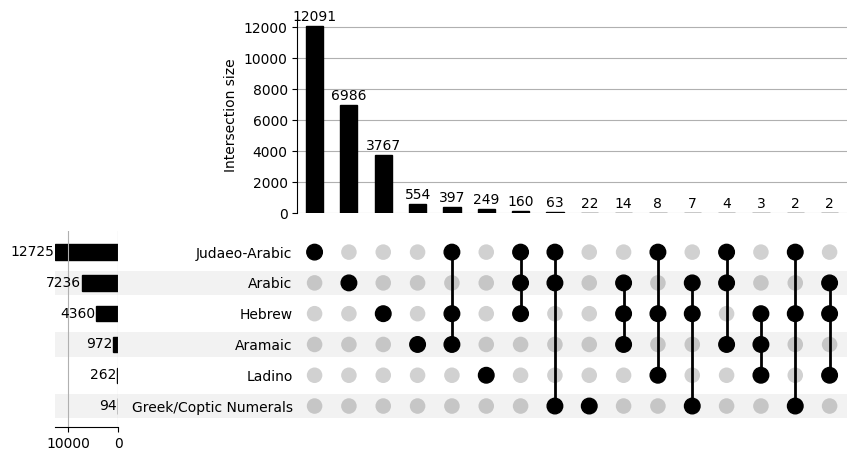
\includegraphics[width=0.8\textwidth]{charts/primary_language_upsetplot.png}
  \caption{An UpSet plot of documents by primary languages, including languages that occur at least 200 times.}
    \medskip
    \small
    The upper bar chart shows the number of documents for different groups of languages and language combinations; the bar chart at left shows the size of each language category across all groups. The matrix provides a visual indicator of the categories at left and the combinations represented in the upper bar chart.\footnotemark
  \label{fig:lang_combination_upset_plot}
\end{figure}

\footnotetext{For more on UpSet plots and the challenges of visualizing overlapping combinations when there are more than four sets, read Koeser's \citetitle{koeser_visualizing_2020}.}

We also distinguish between “primary language,” a designation that indicates that most of the document is written in it, and “secondary language” for languages used only incidentally. Some common examples of secondary languages are Arabic addresses on Judaeo-Arabic letters or Greek/Coptic numerals in Judaeo-Arabic letters and accounts. The distinction between a primary and a secondary language is not always clear-cut: the research team hasn't developed a quantitative threshold, which would have slowed data-entry. One researcher's secondary language may be another's primary; and some may argue that the incidental use of Hebrew and Aramaic is inherently part of Judaeo-Arabic, so should not be marked as secondary languages at all. In practice, as well, whether researchers structure secondary languages depends on their language proficiency and attention to detail, and even seasoned geniza researchers may miss some code-switching, since they are so accustomed to it. These categories could be reviewed and firmed up in the future, perhaps with the help of HTR or other machine learning–based philological tools.

\subsection{Dates and Calendars}

Geniza documents date from the ninth century to the early twentieth, but they are not evenly distributed. Most documents come from the eleventh, twelfth and thirteenth centuries, with significant later clusters from the sixteenth and nineteenth that have received less attention than they deserve.

Situating documents chronologically is essential for historians; it allows them to interpret and contextualize them more accurately. But fragmentary documents can be challenging to date. Rustow has written elsewhere about the challenges and different types of uncertainty involved in dating geniza documents \autocite{rustow_dating_nodate}. Even texts that contain explicit dates may be incomplete: letters, for example, often include the month and day but omit the year, since it would have been obvious to both sender and recipient. 

When a document explicitly notes the date, we structure it as “date on document” and consider it authoritative. This is not always the precise date on which the document was written, but it is usually close enough to serve as a reference point. Documents rarely have more than one date; when they do, we use whichever one is latest. When the document doesn't note the date explicitly, it can sometimes be inferred based on the people, events or types of coins that it mentions (many coins were minted and circulated in limited periods \autocite{dudley_coins_2023}). Many experienced geniza scholars can infer the dates of documents based on handwriting, either because an individual’s hand is well-known or because a style of handwriting occurred only in a certain period. Examples include the scribe Ḥalfon b. Menashshe, a Jewish legal clerk in Fustat active in the first half of the twelfth century, has a distinctive handwriting that allows for confident document dating \autocite{elbaum_halfon_nodate}; and a highly cursive Iberian style of writing that became common in Egypt starting in the late fifteenth century.

\begin{figure}[!hbt]
  \centering
  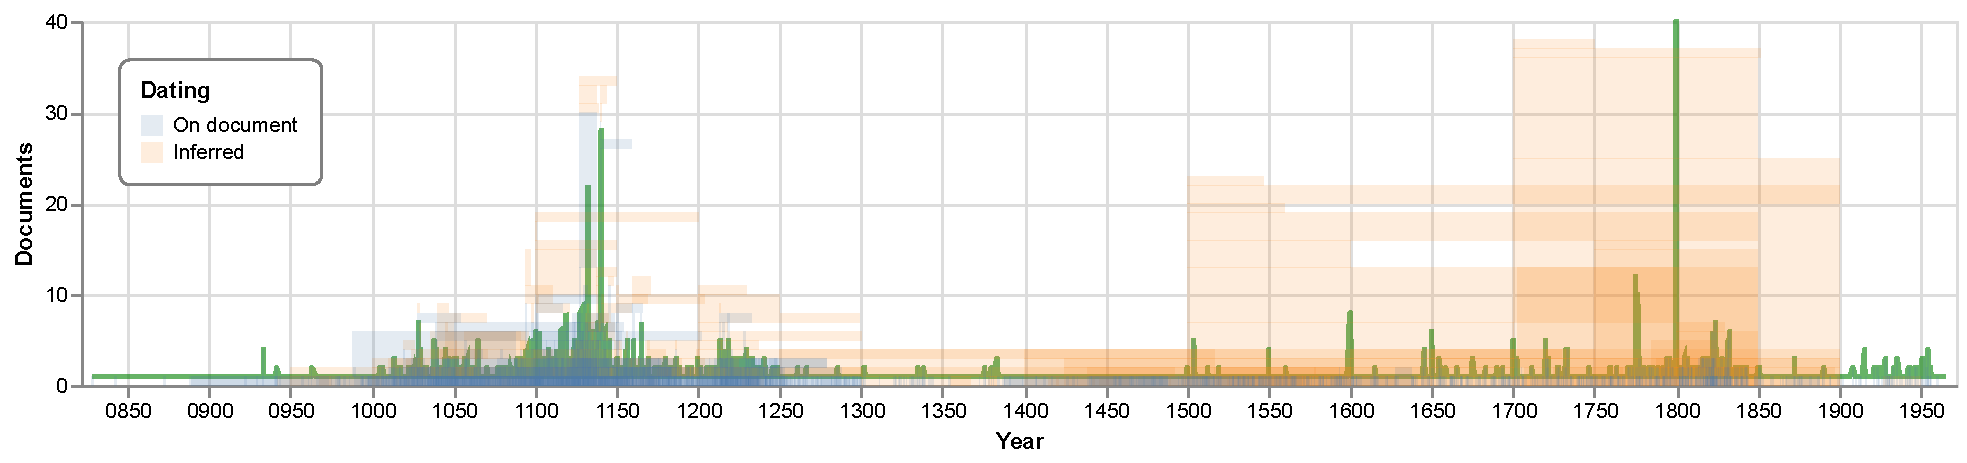
\includegraphics[width=\textwidth]{charts/combined_dating.pdf}
  \caption{Documents by date. The green line chart graphs the totals for documents by year, based on a midpoint date for date ranges. The partial transparent blocks indicate totals for dated documents aggregated by date range.}
  \label{fig:docs_dating_combined}
\end{figure}


The PGP currently has \totalDatedDocs\space dated documents, of which \totalDateOnDoc\space contain an explicit date and \totalInferredDate\space have been dated inferentially.  

Most of the surviving dates on documents use non-Gregorian calendars. These include Jewish (\textit{anno mundi}),  Seleucid, Islamic (\textit{hijrī}) and the Egyptian fiscal calendar (\textit{kharājī}). Months include the Jewish, Coptic and Islamic months, and sometimes a single date will mix and match calendars.\footnote{For instance, a document dated "23 Ḥeshvan (Shawwāl) 521 AH";  the description notes that "it is unusual but not unheard of to combine Hebrew months with the Hijrī calendar" \autocite{noauthor_legal_1127} .} 

Starting with version 4.5 (June 2022), PGPv4 automatically parses and converts Seleucid, \textit{hijrī} and \textit{anno mundi} dates to Common Era dates (Julian before 1583, Gregorian after).\footnote{Calendar conversion is implemented using the Python \texttt{convertdate} library, with additional logic to handle the Seleucid calendar.} Converting to a common calendar enables documents to be sorted, filtered, and compared in a unified chronology, and to be understood by non-expert audiences. (Before June 2022 and the launch of the automated conversion, researchers converted the date using one of several online conversion algorithms such as https://www.muqawwim.com. 

\begin{figure}[!hbt]
  \centering
  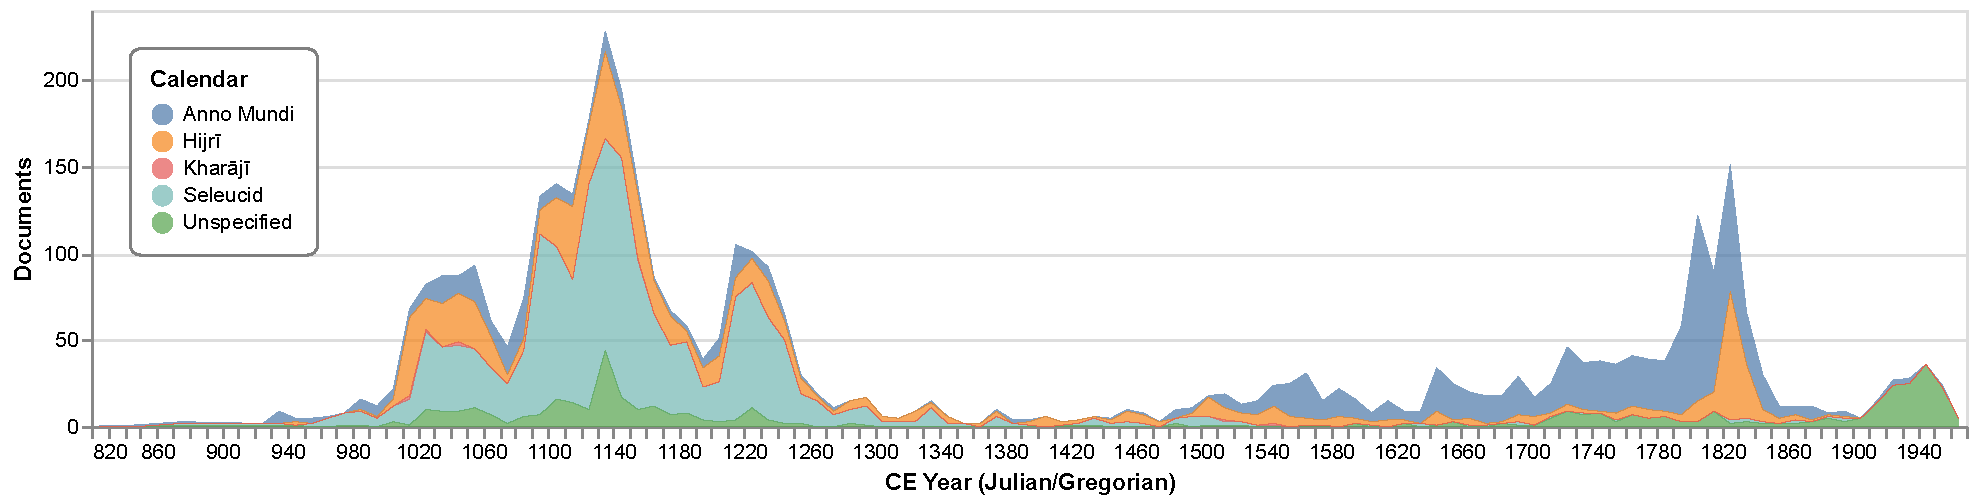
\includegraphics[width=\textwidth]{charts/dated_docs_by_cal.pdf}
  \caption{Dated documents by calendar.}
  \label{fig:docs_dating_combined}
\end{figure}

Like the PGPv4 web interface, the datasets provide both the original calendar and the converted dates, since they are useful for different kinds of analysis. In the datasets, the "date on document" is comprised of three fields: the original date as written, the original calendar, and the standardized date. Inferred dates are similarly comprised of multiple fields: a display field with textual or human-readable information, a standardized date field, a rationale documenting the basis for the inferred date and an optional notes field to provide more information about the dating. In both cases, standardized date fields use Extended Date Time Format (EDTF) for a single date or date range.

\subsection{Scholarship Records}

One of the driving principles of PGP was that any encounter of a human mind with a geniza document is worth preserving: the material is so challenging that it helps to see prior attempts to understand it, even if they were inconclusive. This same principle seems to have been one of Goitein's motivations for retaining his research notes in such an organized and systematic fashion.\footnote{See Goitein's \citetitle{goitein_involvement_1974}, especially section 4, which in retrospect reads uncannily like a blueprint for PGPv4.} Like other digital humanities projects, PGP is both “a work of scholarship and an instrument of scholarship”: it publishes and builds on existing research while also enabling new research \autocite[2]{kotin_world_2024}.

\begin{wraptable}{r}{2.5in}
\caption{Scholarship sources}
\label{table:scholarship_sources}
\begin{tabular}{lrr}
\toprule
Type & Sources & Footnotes \\
\midrule
Unpublished & 264 & 14,908 \\
Article & 245 & 665 \\
Book & 94 & 6,834 \\
Book Section & 55 & 217 \\
Dissertation & 20 & 934  \\
Blog & 1 & 1 \\
\bottomrule
\end{tabular}
\end{wraptable}
All the more important, then, for the database to distinguish clearly between existing and new research. The PGP builds on a substantial scholarly record of both published and unpublished materials, most notably but not solely Goitein’s transcriptions, translations and index cards. (Goitein produced so many thousands of these that we had to split them into pseudo-volumes in our documentation.) Other scholarship in the database includes books, book chapters, articles, dissertations and blog posts, as well as unpublished transcriptions by Goitein’s students, their students and their students’ students, down to current project researchers (see Table \ref{table:scholarship_sources}). 

The way PGPv4 keeps track of all these research outputs—and unpublished products of scholarly research— is by associating documents with "footnotes," a solution  we adapted from previous projects developed at CDH (\citeyear{koeser_princeton-cdhmep-django_2022, koeser_derrida-django_2021}).\footnote{CDH footnotes modules were originally inspired by Jean Bauer’s approach to database footnotes, which were designed to allow for conflicting evidence, indicating “whether or not that source supports the information in the record” (\citeyear{noauthor_tales_2012}).} Footnotes are implemented with a Django “Generic Foreign Key,” which uses a combination of content type (e.g., document, person, place) and object identifier (e.g., document PGPID, or person or place database id) to link to any record in the database). The Shakespeare and Company Project used this approach to link book-borrowing data to the archival sources from which the information was drawn \autocite[18]{kotin_shakespeare_2022}. For PGPv4, we augmented the footnotes with a document relation field that indicates what information the source provides for this specific document—currently, transcription ("Edition" or "Digital Edition"), translation and/or discussion. In the PGP datasets, the \texttt{sources} data are linked to scholarship records that provide citation information and the number of footnotes associated with that source.

\subsection{Transcriptions and Translations}
Transcriptions have long been the gold standard in documentary \textit{geniza }research. The texts are often difficult to read and  contain unique, historically valuable information not found in other historical repositories. Every word is precious and worth the effort to decipher and preserve. Translations are equally valuable, resolving ambiguities in the original and making sense of unclear syntax. And of course they make the material available to a wider pool of researchers.

The PGPv4 database stores and manages transcriptions and translations in the W3C annotation format with minimal HTML formatting. Annotations are linked to images when they are available. The dataset exports include a plain-text version of the transcription and translation content in the content field of the \texttt{footnotes} data. The document relations "Digital Edition" and "Digital Translation" indicate that a record has a  transcription or translation available. Footnotes that note "Edition" or "Translation" indicate that there is a scholarly source containing a transcription or translation of a document, but the content is not yet available in PGPv4. The language of the translation can be determined based on the language of the associated source, typically English and Hebrew.

Researchers should be mindful that transcriptions and translations include editorial symbols such as square brackets, parentheses, curly brackets, ellipses and double brackets. These are customary in philological transcriptions of historical texts. Over the past century, a set of best practices has evolved for scholarly transcription known as the Leiden conventions. (For instance, square brackets enclose an editor’s suggested reconstruction of missing text, as when the manuscript is torn, faded or abraded.)\footnote{https://en.wikipedia.org/wiki/Leiden\_Conventions} In 2021, the PGP team developed a more streamlined version of the Leiden conventions that it uses for new transcriptions\footnote{Refer to \href{https://docs.google.com/document/d/e/2PACX-1vR8kR4zZdnDZXjoLrYrABZn58PRyzrKfEiixQzE9vAzNfzI4Enxs0jU9KO5rTdiH1ZMTPwfqm31mFuX/pub}{Transcription History and Conventions}}. (Some of the older printed transcriptions included in PGP data follow a slightly different version of the Leiden conventions and not all have been brought into line with new standards.) Computational work on transcription content will likely require removing these indicators as a preprocessing step for most use cases. That said, indications of missing or inferred text may also provide an interesting object of study.

\subsection{Images of Fragments}

It is significantly easier to make sense of geniza documents when you can access the fragments themselves or digital images of them. The visual information contained in a fragment can enable an experienced geniza scholar to determine the genre of the text at a glance, and whether it was an official version of a document or the notes of a scribe preparing to write one. It also allows you to see whether the document is fragmentary and where the lacunae are. Moreover, high-resolution images enable scholars to correct the transcriptions that previous generations had made from photostats, microfilms or the original fragments. For all those reasons, we decided that PGPv4 should include digital images alongside text whenever possible. 

We did this by leveraging International Image Interoperability Framework (IIIF) APIs. IIIF provides interoperable mechanisms and associated tooling to publish, use and reference images and groups of images. It also makes it possible to work with aggregated content managed and preserved by different institutions. Libraries and museums around the world are increasingly adopting IIIF to share digitized content; fortunately for us, the three largest \textit{geniza }collections in the world use IIIF APIs to publish their materials. These include tens of thousands of fragments from the Cambridge University Library, which houses around 200,000 fragments; the 43,000 fragments at the Jewish Theological Seminary (JTS) in New York, which are currently hosted by the Digital Princeton University Library (DPUL); and the 17,000 fragments at the University of Manchester. We expect the remaining collections to be made publicly available online via IIIF over the coming years by the National Library of Israel.

In some cases, our reliance on IIIF required waiting for institutions to migrate older digitized images into modern systems, for example, the\textit{ geniza} materials at the University of Pennsylvania, which were imported into PGPv4 in 2023.  In other cases, IIIF image publication required additional organizational and technical creativity. 

For instance, JTS holds 10.75\% of the geniza, but it is a small institution without the technical infrastructure and staffing to host IIIF images. In this case, by building on the Princeton Geniza Lab’s previous agreements to share JTS materials for research, we developed an agreement enabling the DPUL to host and publish JTS images via IIIF. In another case, the Bodleian Library at the University of Oxford, with more than 12,000 fragments, publishes digitized images and metadata available online with permissive licenses, which enabled us to convert their XML metadata into IIIF manifests and lean on PUL infrastructure to serve the images as IIIF. In yet another case, the University of Manchester images are available as IIIF, but each image is published separately with references to their “obverse” image. Since IIIF allows for remixing, the PGPv4 team wrote scripts to combine these images into the more common structure of one manifest per fragment. These manifests preserve information about original ownership and rights; for images that were already published as IIIF, we reference the original manifest by a \texttt{partOf} relationship.

Whenever images are available in PGPv4, the links are included in the \texttt{fragments} data. Records may include the \texttt{url} and the \texttt{iiif\_url}. The first provides a human-viewable format; the second is a machine-readable version, and it links to a IIIF Presentation JSON manifest. Manifests published on \texttt{princetongenizalab.github.io} are the locally customized or remixed versions we have described in the previous paragraph.

Using IIIF has another advantage: it enables us to display the images of multiple fragments that make up a single document (joins), even when those fragments are held by different institutions. The PGPv4 admin interface allows data curators to suppress, reorder and rotate images in order to display only those relevant to a particular document, and in the correct sequence and orientation (for example, omitting the verso if only the recto is needed). PGP datasets do not yet include this document-centric arrangement of images. We recommend toggling between the datasets and the PGPv4 web interface to view images in context. In the meantime, images are accessible through the fragments associated with a document.

\subsection{People and Places}

The PGP datasets include information about people and places associated with the documentary \textit{geniza }corpus. The data currently includes more than 1,100 people and 300 places, and will continue to grow and add more connections. Information about people and places can fuel the analysis of trade and social networks. It also holds the potential to facilitate the dating of undated documents, as when there is a person with a known lifespan who appears in an undated document. 

People and places can be linked to documents in the database, and also to one another. But the datasets do not currently include those relationships, so they are not yet computationally rich in the way that the rest of the datasets are. The current exports include summary information about the number of related documents, but do not yet provide access to the rich information about the connections between them. We hope that future versions of the datasets will include more details on the rich information connecting people, places and documents.

\subsection{Dataset versioning and frequency of change}

PGPv4 is the site of active, ongoing scholarship as team members describe, categorize, transcribe and publish  their research. The team also occasionally makes larger, collaborative efforts for targeted work, for instance, introducing a new document type and updating document records with that new label, as when the team recently splitting out \textbf{Legal query or responsum} from the larger \textbf{Legal document} category. Likewise, the team regularly prepares batch imports of transcription content from published scholarship. Eventually, they will also ingest a batch import of machine-generated transcriptions from the HTR4PGP project.

\begin{figure}[!hbt]
  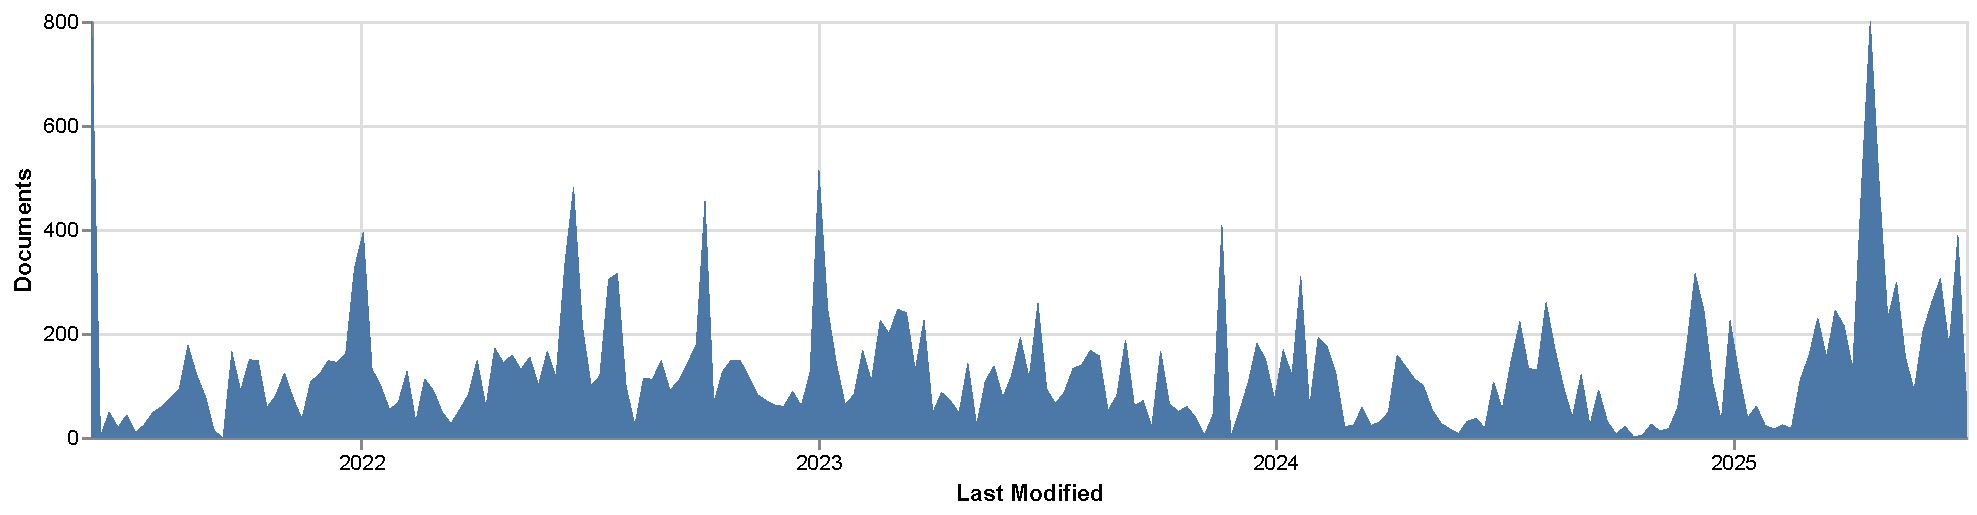
\includegraphics[width=\textwidth]{charts/docs_last_modified.pdf}
  \centering
  \caption{Documents by last modification date.}
  \label{fig:docs-last-modified}
\end{figure}

Both \texttt{documents} and \texttt{fragments} data files include timestamps for the date the record was initially entered and when it was last modified in the database. As a quick analysis shows, hundreds of documents are being modified every week (see Figure \ref{fig:docs-last-modified}). A look at the historic totals of major entities in the PGP datasets shows a steady growth across the data, with occasional jumps enabled by changes in workflow or technology, such as support for transcription editing in PGP version 4.9 (October 2022) or a significant push to work on or import new content.

\begin{figure}[!hbt]
  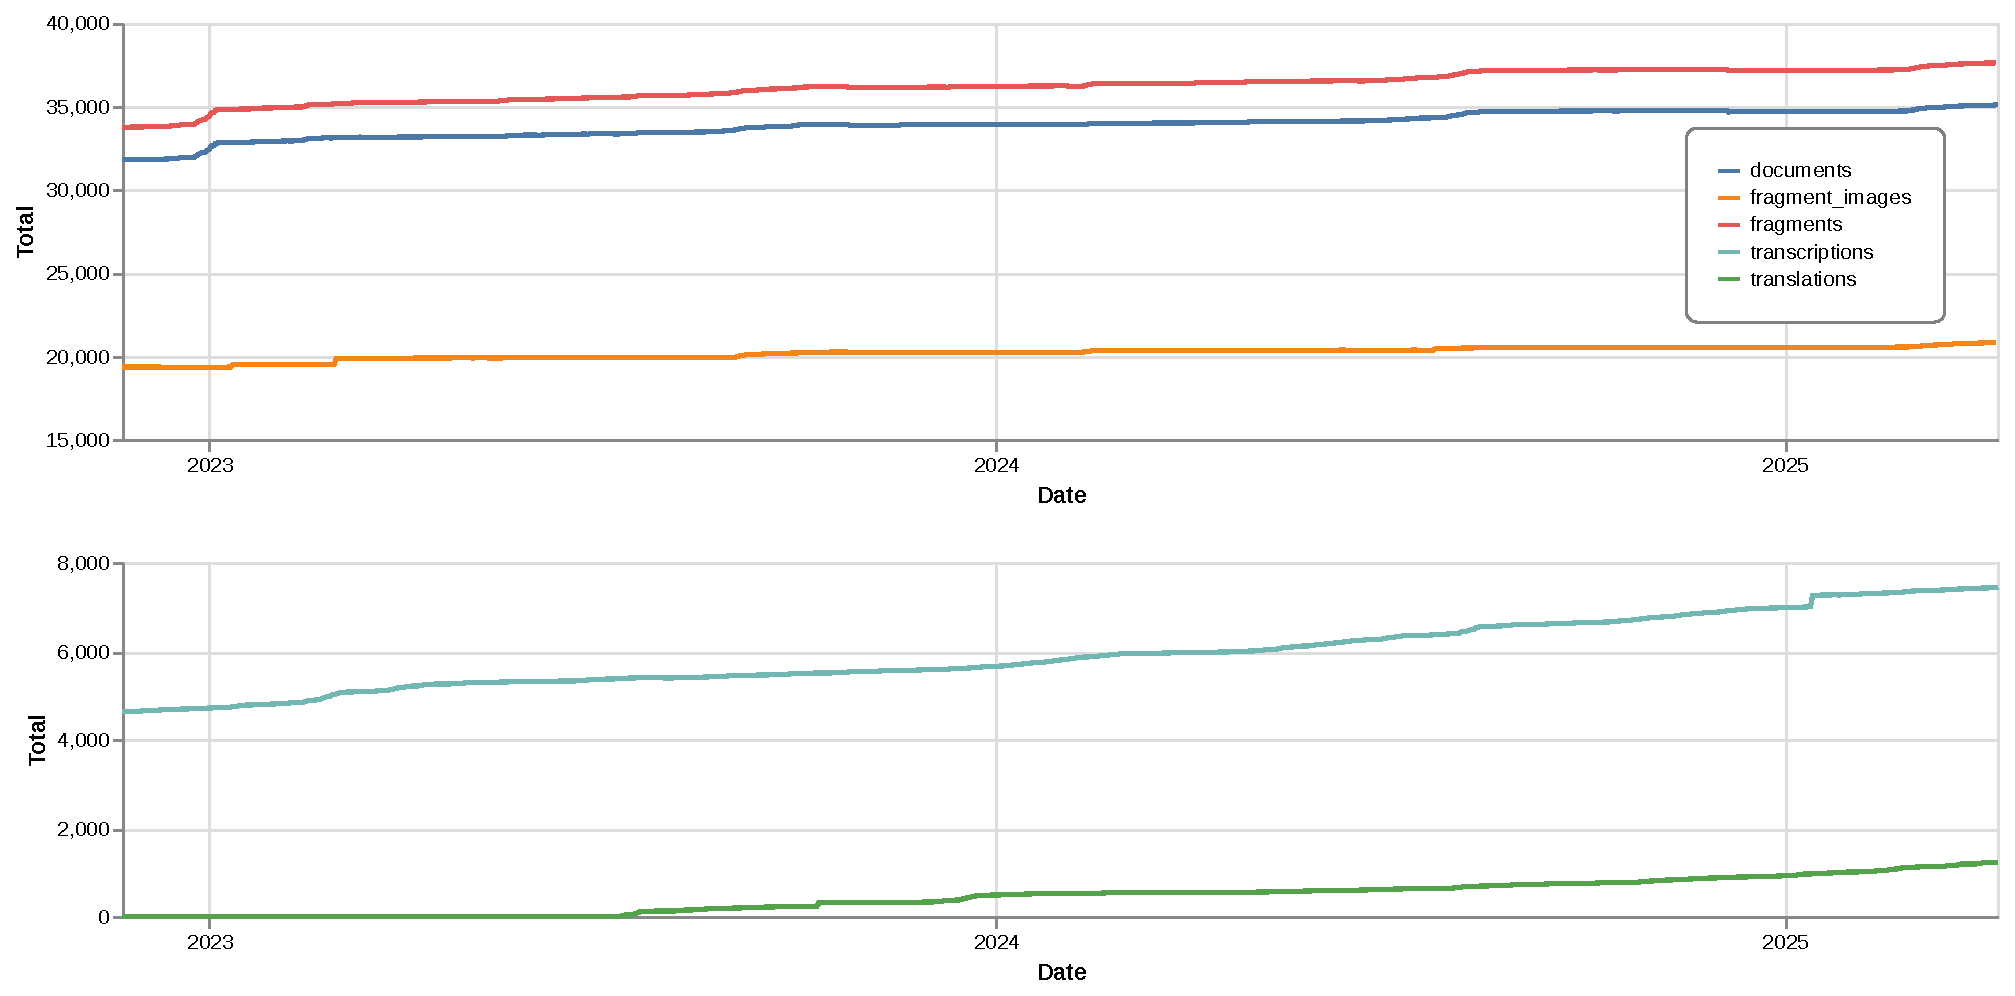
\includegraphics[width=\textwidth]{charts/combined_totals_historic.pdf}
  \centering
  \caption{Historic totals of documents, fragments, images, transcriptions, and translations.}
  \label{fig:historic-totals}
\end{figure}

Because the database is of extraordinarily ancient vintage—forty years is an eternity in digital humanities terms—the datasets include records entered as early as 1986. This longue durée metadata has some potential in itself for analysis.

New versions of the PGP datasets will be published quarterly in order to provide reasonably recent, stable snapshots that can be used for citation and replication, as well as providing larger checkpoints for tracking changes in the long-lived data of a large-scale research project. 

\section{Ongoing and Future Work}

The Cairo Geniza has long had a fascinating, puzzle-box like quality for scholars. Specialists still routinely make new discoveries, some important, some whimsical. Alan Elbaum recently discovered an unknown document written in the handwriting of Moses Maimonides (1138–1204), a philosopher and physician who spent the last forty years of his life in Fustat and is perhaps the most famous Jewish person of the Middle Ages \autocite{ashur_new_2024, noauthor_list_nodate}. Elbaum also discovered a Fatimid government report from 1109 CE about battles with Crusaders during the siege of Tripoli. The fragment provides an astonishing new perspective on a well-known historical event\autocite{elbaum_franks_nodate}. Koeser came across a delightful drawing of a Nile boat (Figure \ref{fig:pgpid8483}) while working on the random sort feature for PGP v4.2 in March 2022; as it turns out, Goitein had known of the fragment, but no one had yet described it in the PGP \autocite{noauthor_paraliterary_nodate}. The development of PGPv4 and the publication of these datasets bear the potential to open up the materials and their many remaining discoveries to work by scholars in new areas of expertise. 

\begin{figure}[!hbt]
  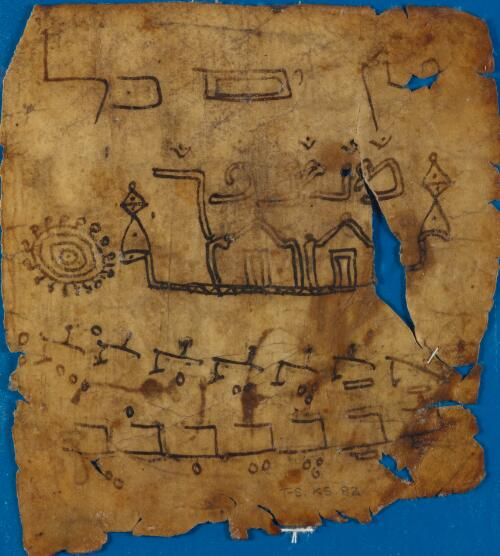
\includegraphics[height=4in]{MS_TS-K-5-2_detail.jpg}
  \centering
  \caption{Recto of T-S K5.82 containing a drawing of a Nile boat \autocite{noauthor_paraliterary_nodate}.}
  \label{fig:pgpid8483}
\end{figure}

The Princeton Geniza Lab is continuing to expand and improve the PGP data, including filing out the People and Places modules and adding new transcriptions and translations. The project has drawn engagement from students eager to work with humanities data and to contribute to active research projects. Undergraduate projects have included network graphs and visualizations, automatic image rotation, Handwritten Text Recognition (HTR), and data cleaning and refinement to help with cataloging efforts. 

An ongoing partnership between Rustow and Daniel Stökl Ben-Ezra \autocite{noauthor_handwritten_nodate} has been leveraging the eScriptorium platform to train and fine-tune HTR models to segment and transcribe PGP materials written in Hebrew script; the project uses the existing PGP scholarly transcriptions as a starting point for training data. The transcriptions these models help generate will eventually be incorporated into the PGPv4 database and datasets, expanding the textual content available for researchers to analyze.

As the amount of full-text content increases, so, too, will the data’s research potential. The need will also become more acute to leverage scalable computational methods, including natural language processing (NLP), machine learning and multimodal language models. One current effort, led by the Princeton Geniza Lab’s research software engineer, Mohamed Abdellatif, is adapting and refining an existing solution for transliterating Judaeo-Arabic to Arabic \autocite{weisberg_mitelman_code-switching_2024}, applying it to PGP transcriptions of Judaeo-Arabic texts to make them more broadly accessible to the Arabic-reading public \autocite{abdellatif_machine_2025}. His effort will also make the content more computationally accessible, since transliteration will allow researchers to work with the material using existing Arabic language models and other NLP tools.

Other projects have also been inspired by PGPv4. Koeser is now leading a collaboration to develop the Python library \texttt{undate} for reasoning with uncertain and partially known dates \autocite{koeser_undate_2024}. This library incorporates and generalizes PGPv4’s solutions for calendar conversion and ambiguous dates, with improved parsing and temporal logic, and may eventually be reintegrated into PGPv4 to improve date handling. It has the potential to make it easier to work with the dates in the PGP datasets and others like them.

Other possibilities include mining specific subsets of PGP materials for information, such as epistolary networks from letters, or analysis of the kinds of legacies inherited through wills. The availability of images in combination with descriptions and transcriptions offers possibilities for multimodal analysis, such as clustering documents visually to identify similar scribal characteristics or individual hands, or identifying other unsuspected commonalities across the materials. PGP images bear further analysis, and torn fragments could be digitally restored either within the PGPv4 or based on future versions of the dataset that provide access to document-centric arrangements of images. Analysis of PGP data in combination with other datasets and sources, such as the historic coins identified by Dudley and Elbaum or the historical places in the World Historical Gazetteer, offers yet more opportunities for new discoveries.

Finally, as a long-running project, the PGP data also offers possibilities for meta-analysis of digital research projects: how have the affordances of changing technologies affected data entry? Tagging and description by researchers with particular interests have resulted in some unevenness of the data, but are footprints detectable across the archive that surface some details but miss others? How will the integration of machine-generated transcription transform PGP research?

By publishing and writing about the PGP datasets, we hope to open up the documentary geniza puzzle box for a new set of scholars and new modes of inquiry. We look forward to seeing what new discoveries will be made by cultural analysts and digital and computational humanities researchers, and to the fruitful interchange between scholars with different domain expertise and training.

\pagebreak
\defbibnote{preamble}

\printbibliography[prenote={preamble}]

\end{document}
